% -- Anfang Präambel
\documentclass[german,  % Standardmäßig deutsche Eigenarten, englisch -> english
parskip=full,  % Absätze durch Leerzeile trennen
%bibliography=totoc,  % Literatur im Inhaltsverzeichnis (ist unüblich)
%draft,  % TODO: Entwurfsmodus -> entfernen für endgültige Version
]{scrartcl}
\usepackage[utf8]{inputenc}  % Kodierung der Datei
\usepackage[T1]{fontenc}  % Vollen Umfang der Schriftzeichen
\usepackage[ngerman]{babel}  % Sprache auf Deutsch (neue Rechtschreibung)

% Mathematik und Größen
\usepackage{amsmath}
\usepackage[locale=DE,  % deutsche Eigenarten, englisch -> US
separate-uncertainty,  % Unsicherheiten seperat angeben (mit ±)
]{siunitx}
\usepackage{physics}  % Erstellung von Gleichungen vereinfachen
\usepackage{yfonts}  % Frakturschrift für Real- und Imaginärteil komplexer Größen

\usepackage{graphicx}  % Bilder einbinden \includegraphics{Pfad/zur/Datei(ohne Dateiendung)}
\usepackage{svg}

% Gestaltung
%\usepackage{microtype}  % Mikrotypographie (kann man am Ende verwenden)
\usepackage{booktabs}  % schönere Tabellen
%\usepackage[toc]{multitoc}  % mehrspaltiges Inhaltsverzeichnis
\usepackage{csquotes}  % Anführungszeichen mit \enquote
\usepackage{caption}  % Anpassung der Bildunterschriften, Tabellenüberschriften
\usepackage{subcaption}  % Unterabbildungen, Untertabellen, …
\usepackage{enumitem}  % Listen anpassen
\setlist{itemsep=-10pt}  % Abstände zwischen Listenpunkten verringern

% Manipulation des Seitenstils
\usepackage{scrpage2}
% Kopf-/Fußzeilen setzen
\pagestyle{scrheadings}  % Stil für die Seite setzen
\clearscrheadings  % Stil zurücksetzen, um ihn neu zu definieren
\automark{section}  % Abschnittsnamen als Seitenbeschriftung verwenden
\ofoot{\pagemark}  % Seitenzahl außen in Fußzeile
\ihead{\headmark}  % Seitenbeschriftung mittig in Kopfzeile
\setheadsepline{.5pt}  % Kopzeile durch Linie abtrennen

\usepackage[hidelinks]{hyperref}  % Links und weitere PDF-Features

% TODO: Titel und Autor, … festlegen
\newcommand*{\titel}{Supraleitung II}
\newcommand*{\autor}{Tom Drechsler, Konstantin Schmid}
\newcommand*{\abk}{SU II}
\newcommand*{\betreuer}{Dr. Sergey Granovsky}
\newcommand*{\messung}{16. Januar 2020}
\newcommand*{\ort}{REC/D008}

\hypersetup{pdfauthor={\autor}, pdftitle={\titel}}  % PDF-Metadaten setzen

% automatischen Titel konfigurieren
\titlehead{Fortgeschrittenen-Praktikum \abk \hfill TU Dresden}
\subject{Versuchsprotokoll}
\title{\titel}
\author{\autor}
\date{\begin{tabular}{ll}
Protokoll: & \today\\
Messung: & \messung\\
Ort: & \ort\\
Betreuer: & \betreuer\end{tabular}}

% -- Ende Präambel

\begin{document}
\begin{titlepage}
\maketitle  % Titel setzen
\tableofcontents  % Inhaltsverzeichnis
\end{titlepage}

% Text Anfang
\section{Versuchsziel und Überblick}
In diesem Versuch ist die Abhängigkeit des kritischen Magnetfeldes, bei dem der Übergang von Supraleitung zur Normalleitung erfolgt, zu untersuchen. Weiterhin soll der Versuch Kenntnisse und Fähigkeiten zum Aufbau von Tieftemperatur-Kryostaten und zur Handhabung kryogener Kältemittel (LHe, L$\text{N}_2$) vermitteln. Dazu sind folgende Versuchsteile zu bearbeiten:
\begin{itemize}
\item Einkühlen eines LHe-Badkryostaten
\item Bestimmung des kritischen Magnetfeldes für eine Blei-Probe als Funktion der Temperatur im Temperaturbereich zwischen $1.5$ K und $10$ K
\item Konstruktion der Phasenlinie zwischen supraleitendem und normalleitendem Zustand und Vergleich mit der BCS-Theorie und Literaturwerten
\end{itemize}

\section{Theoretische Grundlagen}
\subsection{Supraleitung}
Bei supraleitenden Materialien tritt bei einer kritischen Temperatur T$_{\text{C}}$ (gleichbedeutend mit Sprungtemperatur) ein Phasenübergang vom normalleitenden Zustand zum supraleitenden Zustand auf. Dieser ist dann  dadurch gekennzeichnet, dass der Gleichstromwiderstand auf $0$ abfällt oder er zumindest so nahe bei $0$ liegt, dass in supraleitenden Ringen Dauerströme beobachtet werden können. (\cite{5}, Seite 371)
\newpage
Dies ist in Abbildung 1 für Quecksilber dargestellt.
\\
\begin{figure}[h!]
\centering
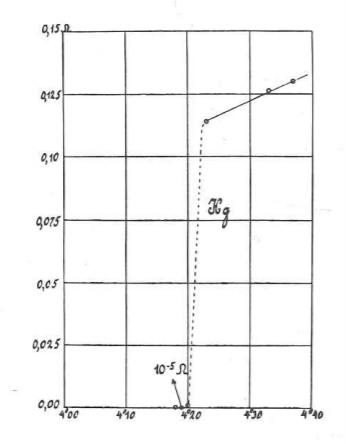
\includegraphics[width=0.5\textwidth]{hg}
\caption{Verhalten des Widerstandes eines Supraleiters bei verschiedenen Temperaturen, entnommen aus \cite{5} (Seite 370).}
\end{figure}
\subsubsection{Auftreten der Supraleitung}
Supraleitung kann bei verschiedenen Arten von Materialien auftreten: bei vielen metallischen Elementen, Legierungen, intermetallischen Verbindungen und Halbleitern. Dabei können verschiedene Sprungtemperaturen beobachtet werden. Auftretende Werte für T$_{\text{C}}$ erstrecken sich von $0.001$ K für Rhodium bis $250$ K für LaH$_{10}$.  Supraleiter, die so eine signifikant höhere Sprungtemperatur besitzen, werden als Hochtemperatursupraleiter bezeichnet.
\newpage
In diesem Versuch wird Blei untersucht. Der Literaturwert für die kritische Temperatur für Blei liegt bei T$_{\text{C}} = 7.196$ K. Dies kann aus Abbildung 2 entnommen werden.
\begin{figure}[h!]
\centering
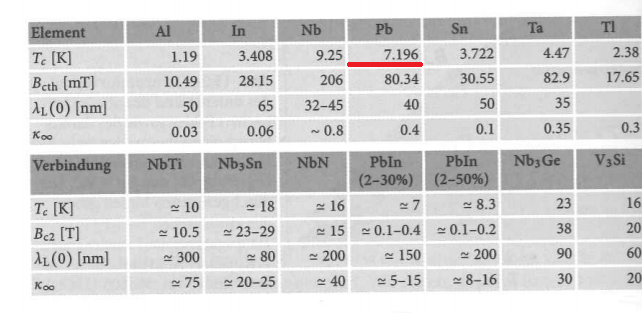
\includegraphics[width=0.95\textwidth]{tab}
\caption{Kritische Temperaturen einiger Supraleiter, entnommen aus \cite{6} (Seite 816).}
\end{figure}

\subsubsection{BCS-Theorie}
Die BCS-Theorie liefert die theoretische Erklärung zur Entstehung der konventionellen Supraleitung:
\\\\
Ein Elektron verändert durch Energieabgabe die Gitterschwingung, sodass ein zweites Elektron durch Aufnahme eines Phonons einen dementsprechenden Energiegewinn erzielt. Diese beiden Elektronen können nun ein sogenanntes Cooper-Paar bilden. Dieses hat die Eigenschaft, dass es bosonischen Charakter hat, da Elektronen Fermionen mit Spin $s = \frac{1}{2}$ sind. Bei gleicher Richtung der Spins der Elektronen im Cooper-Paar erhält man also einen Gesamtspin $S=1$ und bei entgegen gerichteten Spins $S=0$. Bosonen können beliebig häufig den gleichen Zustand besetzen, so auch den Grundzustand. Dies ist energetisch günstiger und kann mit Hilfe einer Bose-Einstein-Wellenfunktion mathematisch beschrieben werden. Die Wellenfunktion überspannt den gesamten Festkörper und kann so von lokalen Hindernissen nicht mehr beeinflusst werden, sodass ein widerstandsloser Ladungstransport möglich ist.
\\\\
Das Problem an dieser Theorie ist, dass durch den Ausgangspunkt der Veränderung der Gitterschwingung durch Elektronen die Temperatur sehr gering sein muss. Somit können mit der Theorie in der hier dargestellten Form keine Hochtemperatur-Supraleiter beschrieben werden, die deshalb auch als unkonventionelle Supraleiter bezeichnet werden.

\subsubsection{Zerstörung der Supraleitung durch Magnetfelder}
Durch genügend große Magnetfelder kann der Effekt der Supraleitung zerstört werden. Das Magnetfeld, bei dem dieser Übergang erfolgt, wird als H$_{\text{C}}$(T) (kritisches Magnetfeld) bezeichnet. Dieses ist temperaturabhängig und hat bei der kritischen Temperatur den Wert $0$. Für H$_{\text{C}}$(T) gilt folgender Zusammenhang:
\begin{align}
\label{h}
\text{H}_{\text{C}}(\text{T}) = \text{H}_{\text{C,0}}( \text{T}) \, \left[1-\left(\frac{\text{T}}{\text{T}_{\text {C}}}\right)^2 \right].
\end{align}
Die Strategie in diesem Versuch ist es also für verschiedene Temperaturen das kritische Magnetfeld zu messen und so das Phasendiagramm zu konstruieren. Der zu erwartende Verlauf im Phasendiagramm ist in Abbildung 3 dargestellt:
\begin{figure}[h!]
\centering
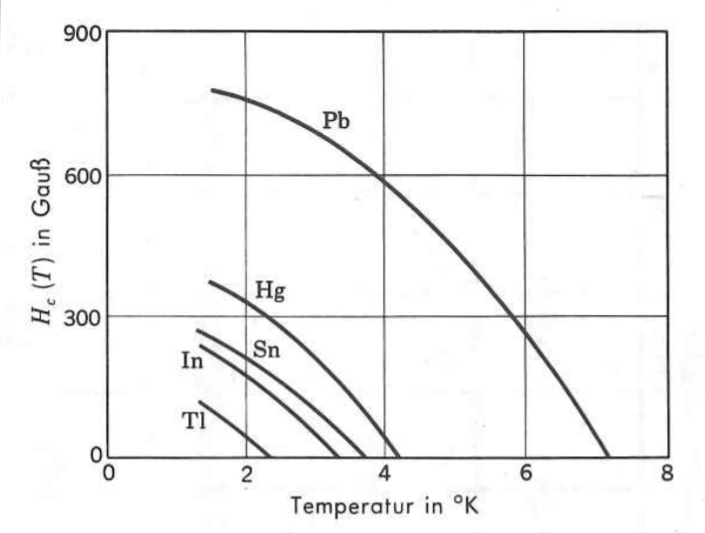
\includegraphics[width=0.57\textwidth]{pd_kittel}
\caption{Phasendiagramm mit kritischen Magnetfeldern verschiedener Supraleiter, entnommen aus \cite{5} (Seite 374).}
\end{figure}
\newpage
Die durchgezogenen Linien sind die kritischen Magnetfelder, also die Schwellenwerte. Links unterhalb dieser ist der supraleitende Zustand, rechts oberhalb sind die Materialien normalleitend.

\subsection{Magnetfeld einer Spule}
Das Magnetfeld, welches in diesem Versuch verwendet wird, wird durch eine Spule erzeugt. Allgemein erhält man solche Magnetfelder durch das Biot-Savart-Gesetz:
\begin{align}
\text{d}\vec{B}(\vec{r}) = \frac{\mu_{0}}{4\pi} \, I \, \text{d}l \times \frac{\vec{r}- \vec{r}'}{|\vec{r}- \vec{r}'|^3}.
\end{align}
Ausführen dieser Rechnung für eine Zylinderspule führt auf:
\begin{align}
B(0) = \mu_{0} \frac{N\,I}{\sqrt{(2R)^2+l^2}}.
\end{align}
$N$ bezeichnet hierbei die Windungszahl der Spule, $I$ die Stromstärke, $R$ den Radius der Spule und $l$ die Länge der Spule. Da bei der uns vorliegenden Kupfer-Spule $l \gg 2R$ gilt, kann folgender Näherungsausdruck für das erzeugte Magnetfeld verwendet werden:
\begin{align}
\label{b}
B \approx \mu_{0} \, \frac{N \, I}{l}.
\end{align}
Um gegebenenfalls $H$ und nicht $B$ zu betrachten, muss Gleichung (\ref{b}) noch durch $\mu_0$ geteilt werden:
\begin{align}
H = \frac{N \, I}{l}.
\end{align}
Der Faktor $\frac{N}{l}$ ist dabei als $234  \, \frac{1}{\text{cm}}$ vorgegeben. So kann im Versuch das Magnetfeld durch Variieren der Stromstärke eingestellt werden.

\subsection{Das Ge-Thermometer}
Im Versuch wird ein Ge-Thermometer verwendet. Bei diesem wird über den Widerstand die Temperatur bestimmt. Der Vorteil bei dieser Methode ist, dass das Signal direkt als Spannung vorliegt und über das Ohm'sche Gesetz in einen Widerstand umgerechnet werden kann:
\begin{align}
R = \frac{U}{I}.
\end{align} 
Es bietet sich in diesem Versuch die Verwendung von Germanium an, da dieses ein Halbleiter ist. Die qualitative Darstellung des Widerstandes eines Halbleiters in Abhängigkeit von der Temperatur ist in Abbildung 4 beispielhaft illustriert.
\\\\\\
\begin{figure}[h!]
\centering
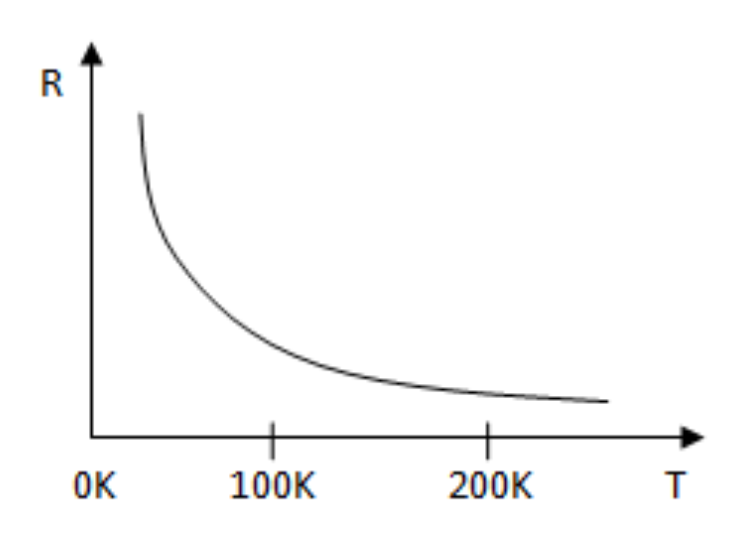
\includegraphics[width=0.55\textwidth]{res_sc}
\caption{Widerstand eines Halbleiters, entnommen aus \cite{4}.}
\end{figure}
\\\\
Es ist vor allem das Verhalten bei kleinen Temperaturen relevant. Für kleine Temperaturen unterscheiden sich die Widerstände aufgrund des exponentiellen Abfalls deutlich, sodass besonders diese Temperaturen gut zu messen sind, was für den Versuch eine wichtige Grundvoraussetzung ist. Für Metalle verläuft die Kurve im betrachteten Temperaturbereich annähernd konstant, sodass der Einsatz eines metallischen Widerstandsthermometers hier nicht funktioniert.

\newpage
\subsection{Versuchsaufbau}
Der verwendete Versuchsaufbau ist in Abbildung 5 dargestellt.
\\\\\
\begin{figure}[h!]
\centering
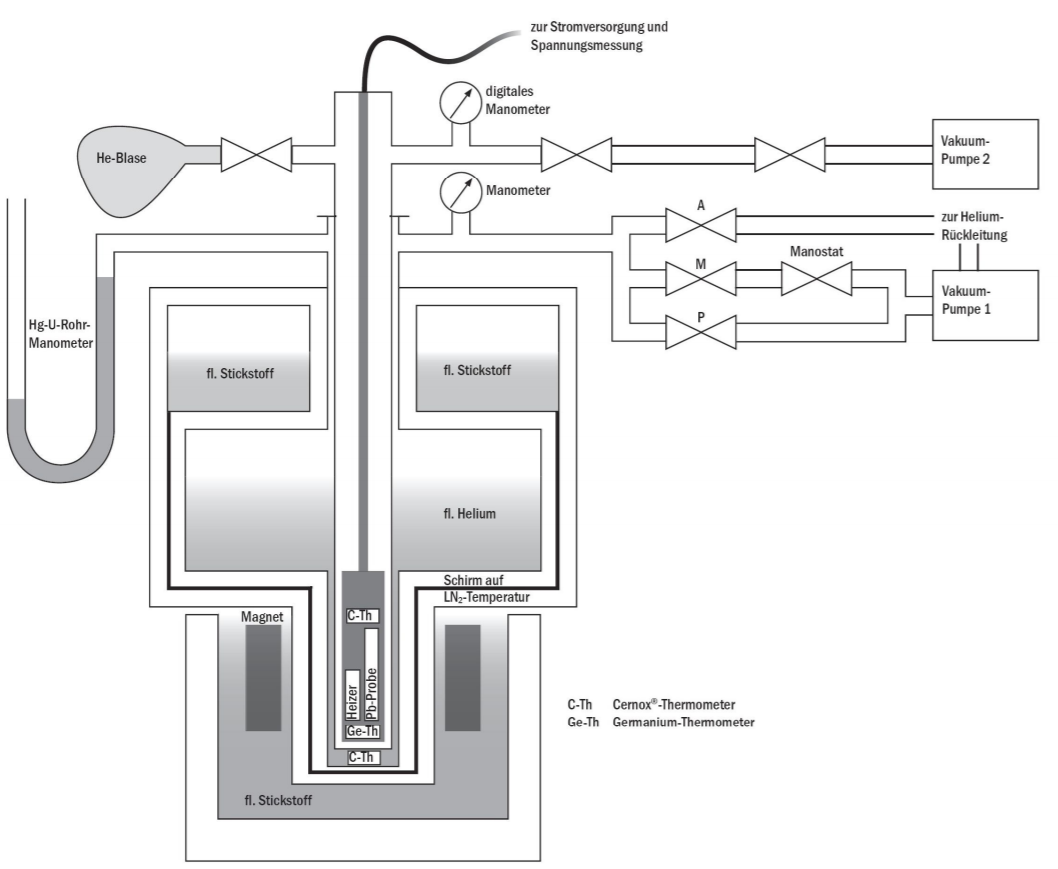
\includegraphics[width=0.7\textwidth]{aufbau}
\caption{Verwendeter Versuchsaufbau, entnommen aus \cite{3}.}
\end{figure}
\\\\
Der Magnet, also die Kupfer-Spule, wird mit Hilfe von flüssigem Stickstoff gekühlt. Die Bleiprobe wird durch flüssigen Stickstoff und flüssiges Helium gekühlt. Da durch diese Kühlung allerdings nur eine Temperatur von $4.2$ K erreicht werden kann, gibt es das Manostat und die Vakuumpumpe 1. Durch diese kann der Druck verändert werden. Durch Abpumpen des Dampfes über der Flüssigkeit (LHe) wird die Temperatur gesenkt, sodass mit diesem Aufbau Temperaturen bis ca. $1.8$ K erreicht werden können. Die Messung des Drucks erfolgt über Manometer. Um Temperaturen über $4.2$ K zu erhalten, ist bei der Bleiprobe ein Heizer vorhanden, der dann die Temperatur auf $10$ K erhöhen kann.
\\\\
Der konkrete Aufbau des Kryostats findet sich in Abbildung 6 wieder.
\begin{figure}[h!]
\centering
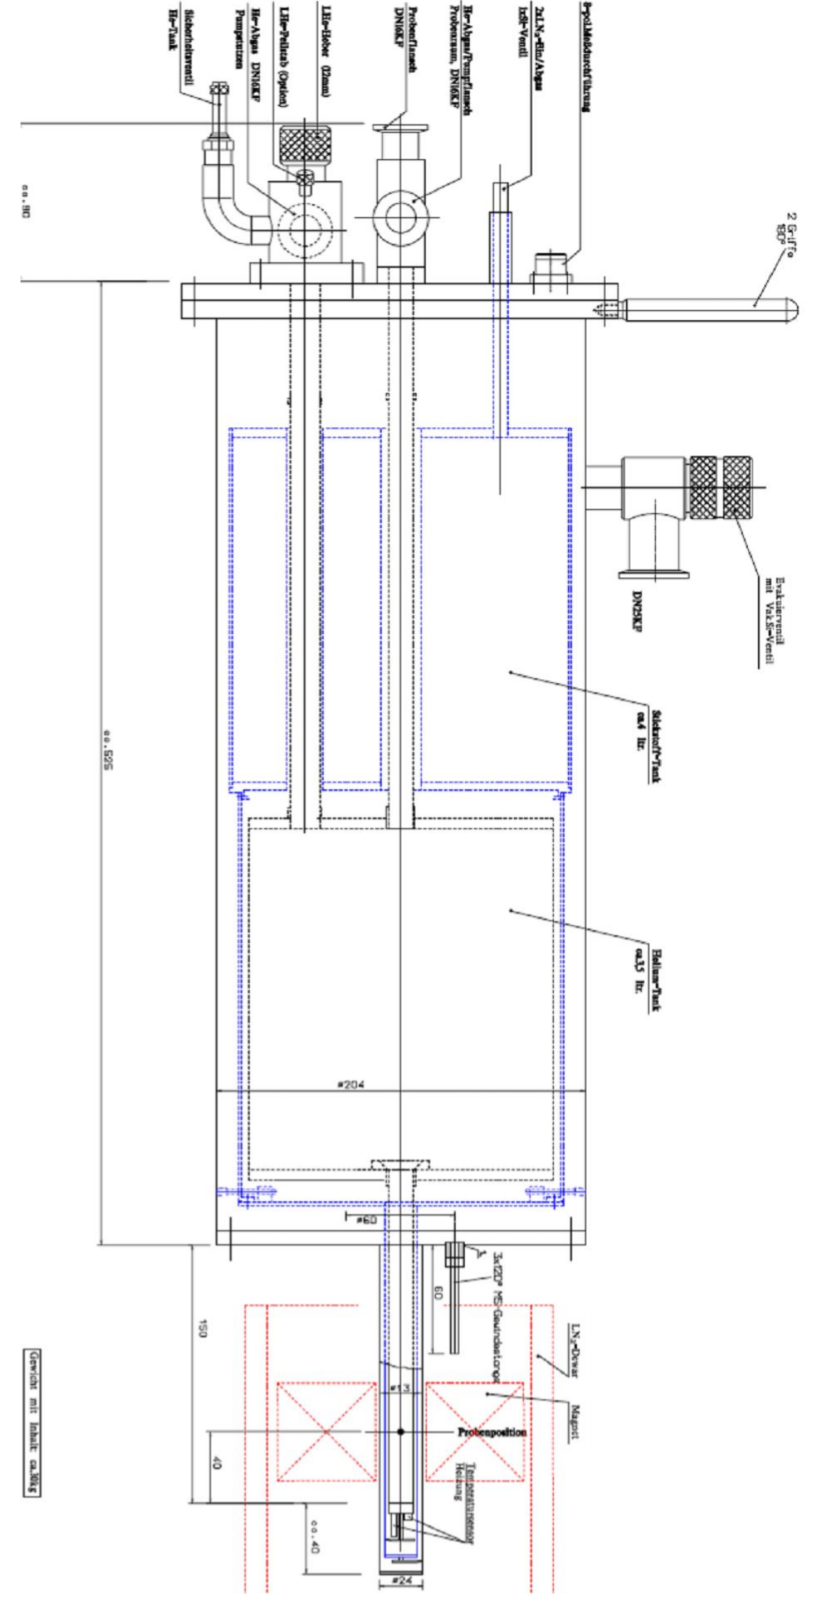
\includegraphics[width=0.51\textwidth]{kryo}
\caption{Aufbau des Kryostats, entnommen aus \cite{3}.}
\end{figure}
\newpage
\section{Durchführung}
\subsection{Abkühlen des Badkryostaten}
\begin{itemize}
\item Einschalten der Messgeräte und Ausschalten des Heizers, um unkontrolliertes Heizen zu vermeiden
\item nach Vakuumieren des Kryostats (vom Betreuer am Vortag erledigt): Einfüllen von flüssigem Stickstoff in Außenbehälter (LN$_{2}$-Drucktank an Gefäß über Teflonschlauch angeschlossen), Einfüllen beendet als LN$_{2}$ am Abgasstutzen herausspritzt
\item nach Erreichen einer Temperatur von unter $150$ K: Einfüllen von flüssigem Helium möglich
\item Einführen des Hebersystems in das Heliumgefäß bzw. in das Kryostat und Verbinden beider Teile, leichtes Öffnen des Ventils am Hebersystem, Ablesen des Wertes der Gasuhr, Beobachten des Laufs der Gasuhr, bei schnellem Lauf der Gasuhr ist durch das Ventil zu drosseln, bei erneut schnellem Lauf der Gasuhr ist das Befüllen zu beenden
\item Abwarten der Abkühlung bis ca. $4.2$ K
\item Kühlen der Spule mit flüssigem Stickstoff, um Durchbrennen der Windungen zu vermeiden: Füllen des Kunststoff-Dewargefäßes mit flüssigem Stickstoff, Schieben des Gefäßes über das Endstück des Kryostaten und Herausziehen des Versuchsstandes zwecks Abstellen des Gefäßes
\item Nachfüllen des Gefäßes mit flüssigem Stickstoff ca. alle $20$ min., da Gefäß nicht ideal isoliert
\end{itemize}

\subsection{Computerfunktion}
\begin{itemize}
\item Einschalten des Computers und Starten des SU-Messprogramms
\item Überprüfung der Messfunktion durch Taste Messen
\item Aufnahme einer ersten Messreihen für $4.2$ K bei Stromstärken von $0$\,A bis $3$\,A
\item Speichern der Daten
\end{itemize}

\subsection{Kritisches Feld einer supraleitenden Bleiprobe für 2.0\,K < T < 4.2\,K}
\begin{itemize}
\item Verringerung der Temperatur durch Abpumpen des Dampfs über der Flüssigkeit (LHe) mit Pumpe 1
\item Aufnahme von ca. 10 Messreihen über:
\begin{itemize}
\item[-] Einschalten der Vakuumpumpe (Pumpe 1), Regulierung des Dampfdrucks über Manostat M (Ventil A geschlossen, Ventil M geöffnet, Ventil P geschlossen)
\item[-] Aufnahme einer Messkurve für jeden Druckwert (Computerprogramm), Variieren des Spulenstroms von $0$\,A bis $3$\,A
\item[-] für letzten Wert längeres Abpumpen um tiefste Temperatur zu vermessen
\end{itemize}
\item nach Beenden der Messreihen: Belüften des LHe-Bades auf Normaldruck (Pumpe aus, Ventil A langsam öffnen) und  Belüften des Manostats (Ventil A offen, Ventil M öffnen, Manostat aufdrehen)
\end{itemize}

\subsection{Kritisches Feld einer supraleitenden Bleiprobe für 4.2\,K < T < 10\,K}
\begin{itemize} 
\item thermisches Abkoppeln der Probe vom LHe-Bad: Abpumpen des Austauschgases, Öffnen der Ventile an der Pumpe und am Kryostaten
\item Erhöhung der Temperatur nun möglich ohne LHe vollständig zu verdampfen
\item Temperaturregelung über LakeShore Temperature Controller: Einstellen des Temperatursollwertes über Setpoint, Einstellen der maximalen Leistung über Heater Range auf $625$\,mW
\item Temperaturerhöhung in Schritten von $0.2$ K
\item Aufzeichnen der Messwerte nach Stabilisierung der Temperatur, wieder Stromstärken von $0$\,A bis $3$\,A
\item Beenden der Messung, wenn bei einer Messreihen kein Sprung mehr auftritt (Probe auch ohne Magnetfeld normalleitend)
\item Ablesen der Gasuhr nach Beenden der Messung
\end{itemize}

\newpage
\section{Auswertung}
\subsection{Vorversuch}
In einem ersten Vorversuch sollte gezeigt werden, dass die aufgenommenen Messdaten für eine gleiche Temperatur unabhängig von der Richtung des Stromes durch die Probe sind. Dazu wurde für T = $4.309$\,K einmal für für I = $0.2$\,A in positive und einmal für die gleiche Stromstärke in negative Richtung vermessen (siehe Abbildung 7). \\\\
\begin{figure}[h!]\centering
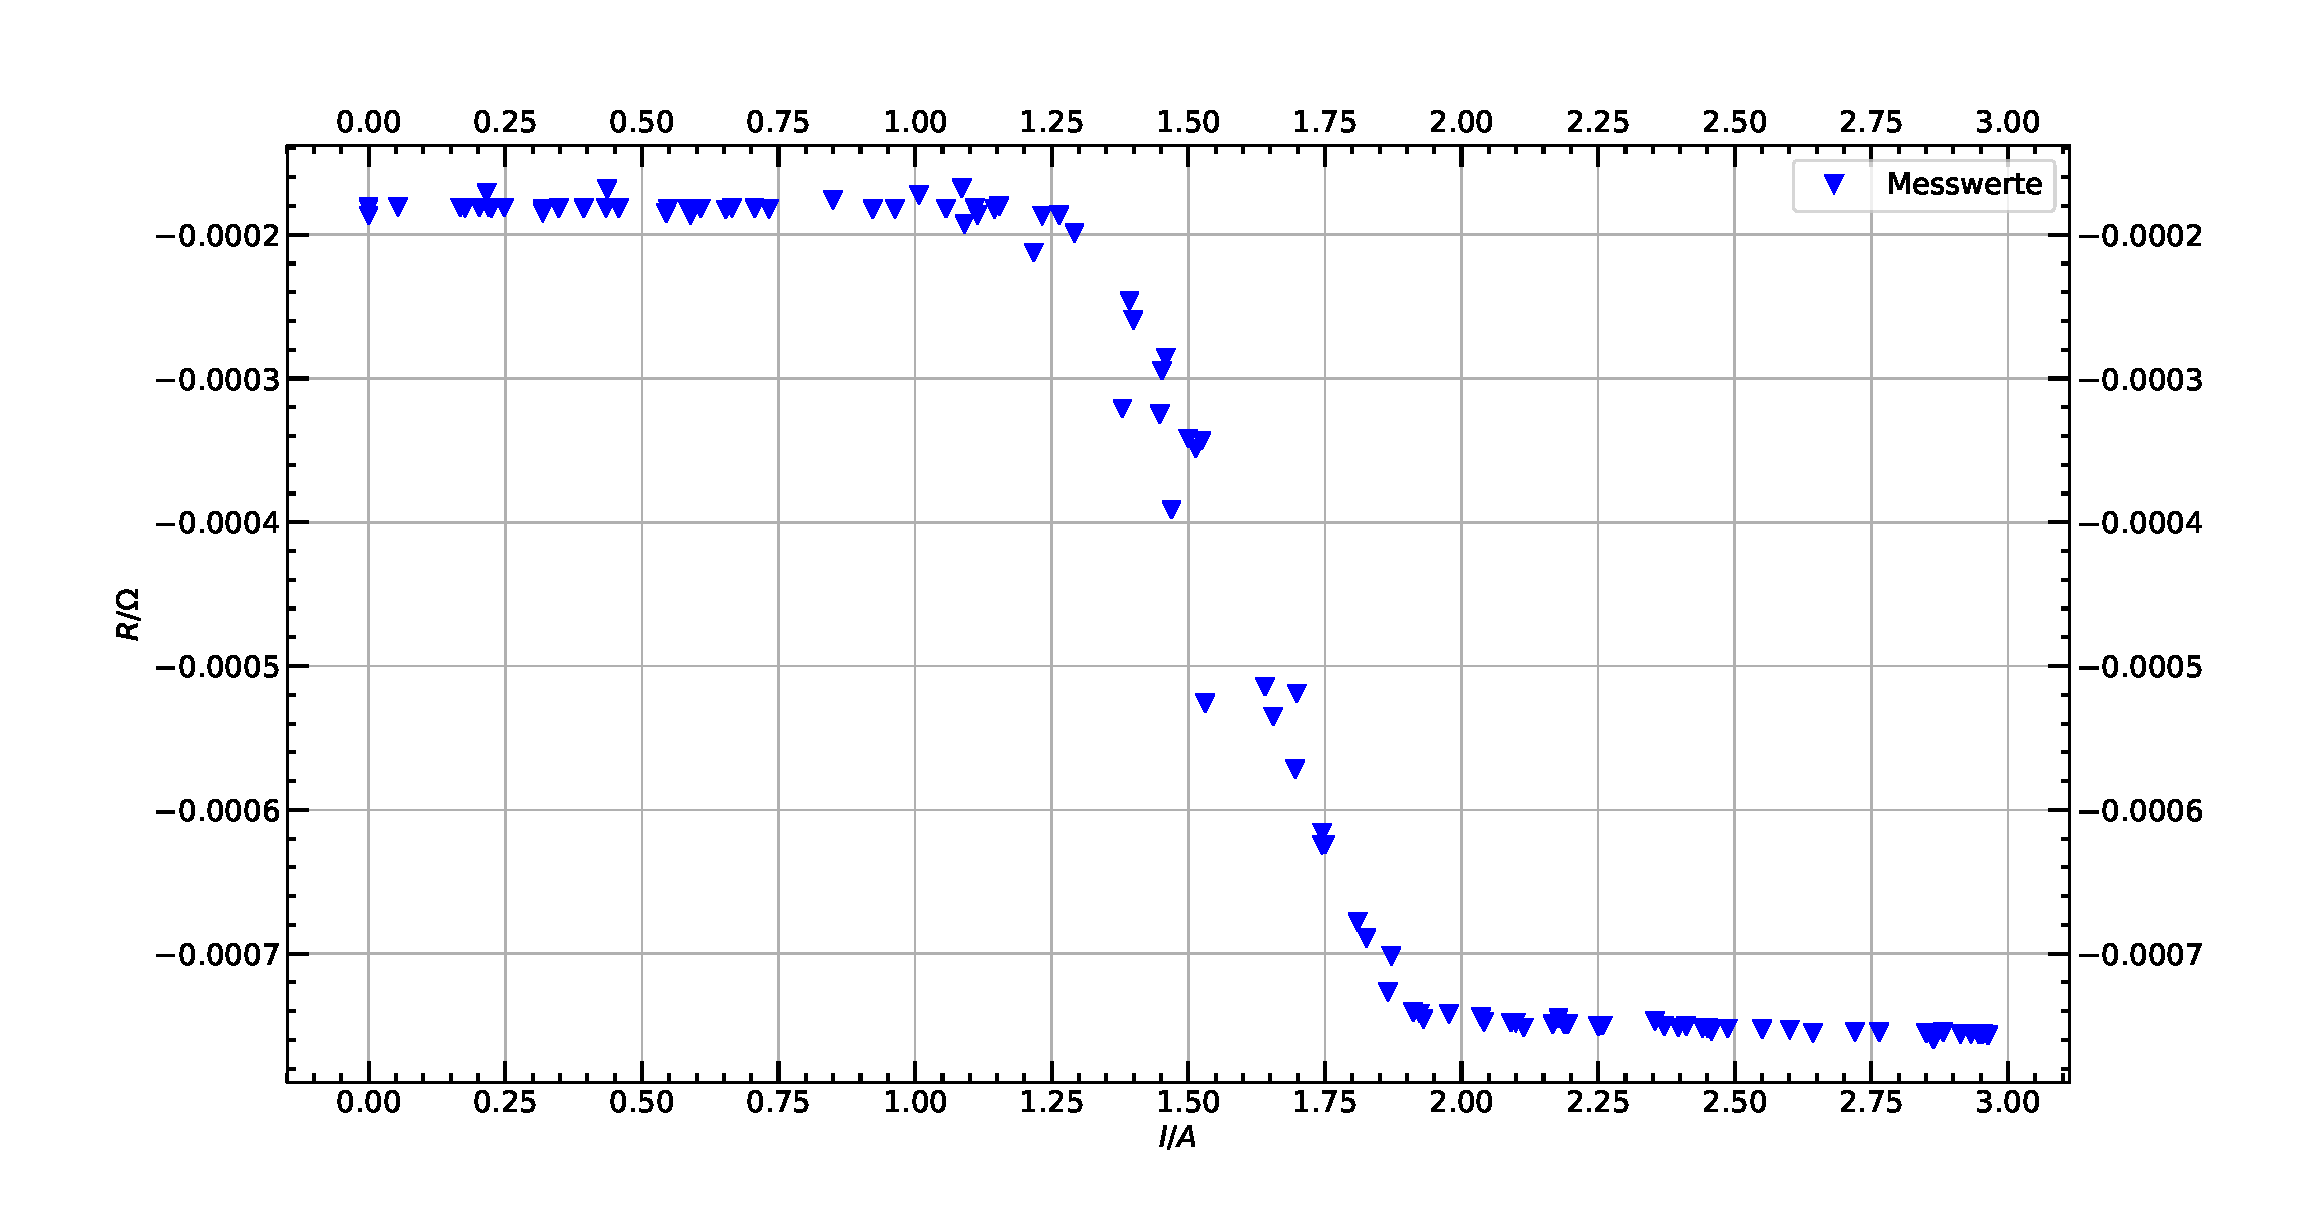
\includegraphics[width=\textwidth]{Vorversuch.pdf}
\caption{Messung in negativer Stromrichtung.}
\end{figure}


Der Verlauf der Kurve ändert sich in negativer Stromrichtung nicht.
\subsection{Bestimmung der kritischen Magnetfelder}
Um die Methode der Auswertung einmal exemplarisch zu erklären wurde die erste Messung (für eine Temperatur von $4.31$\,K) ausgewählt (Abbildung 8).
\newpage
\begin{figure}[h!]
\centering
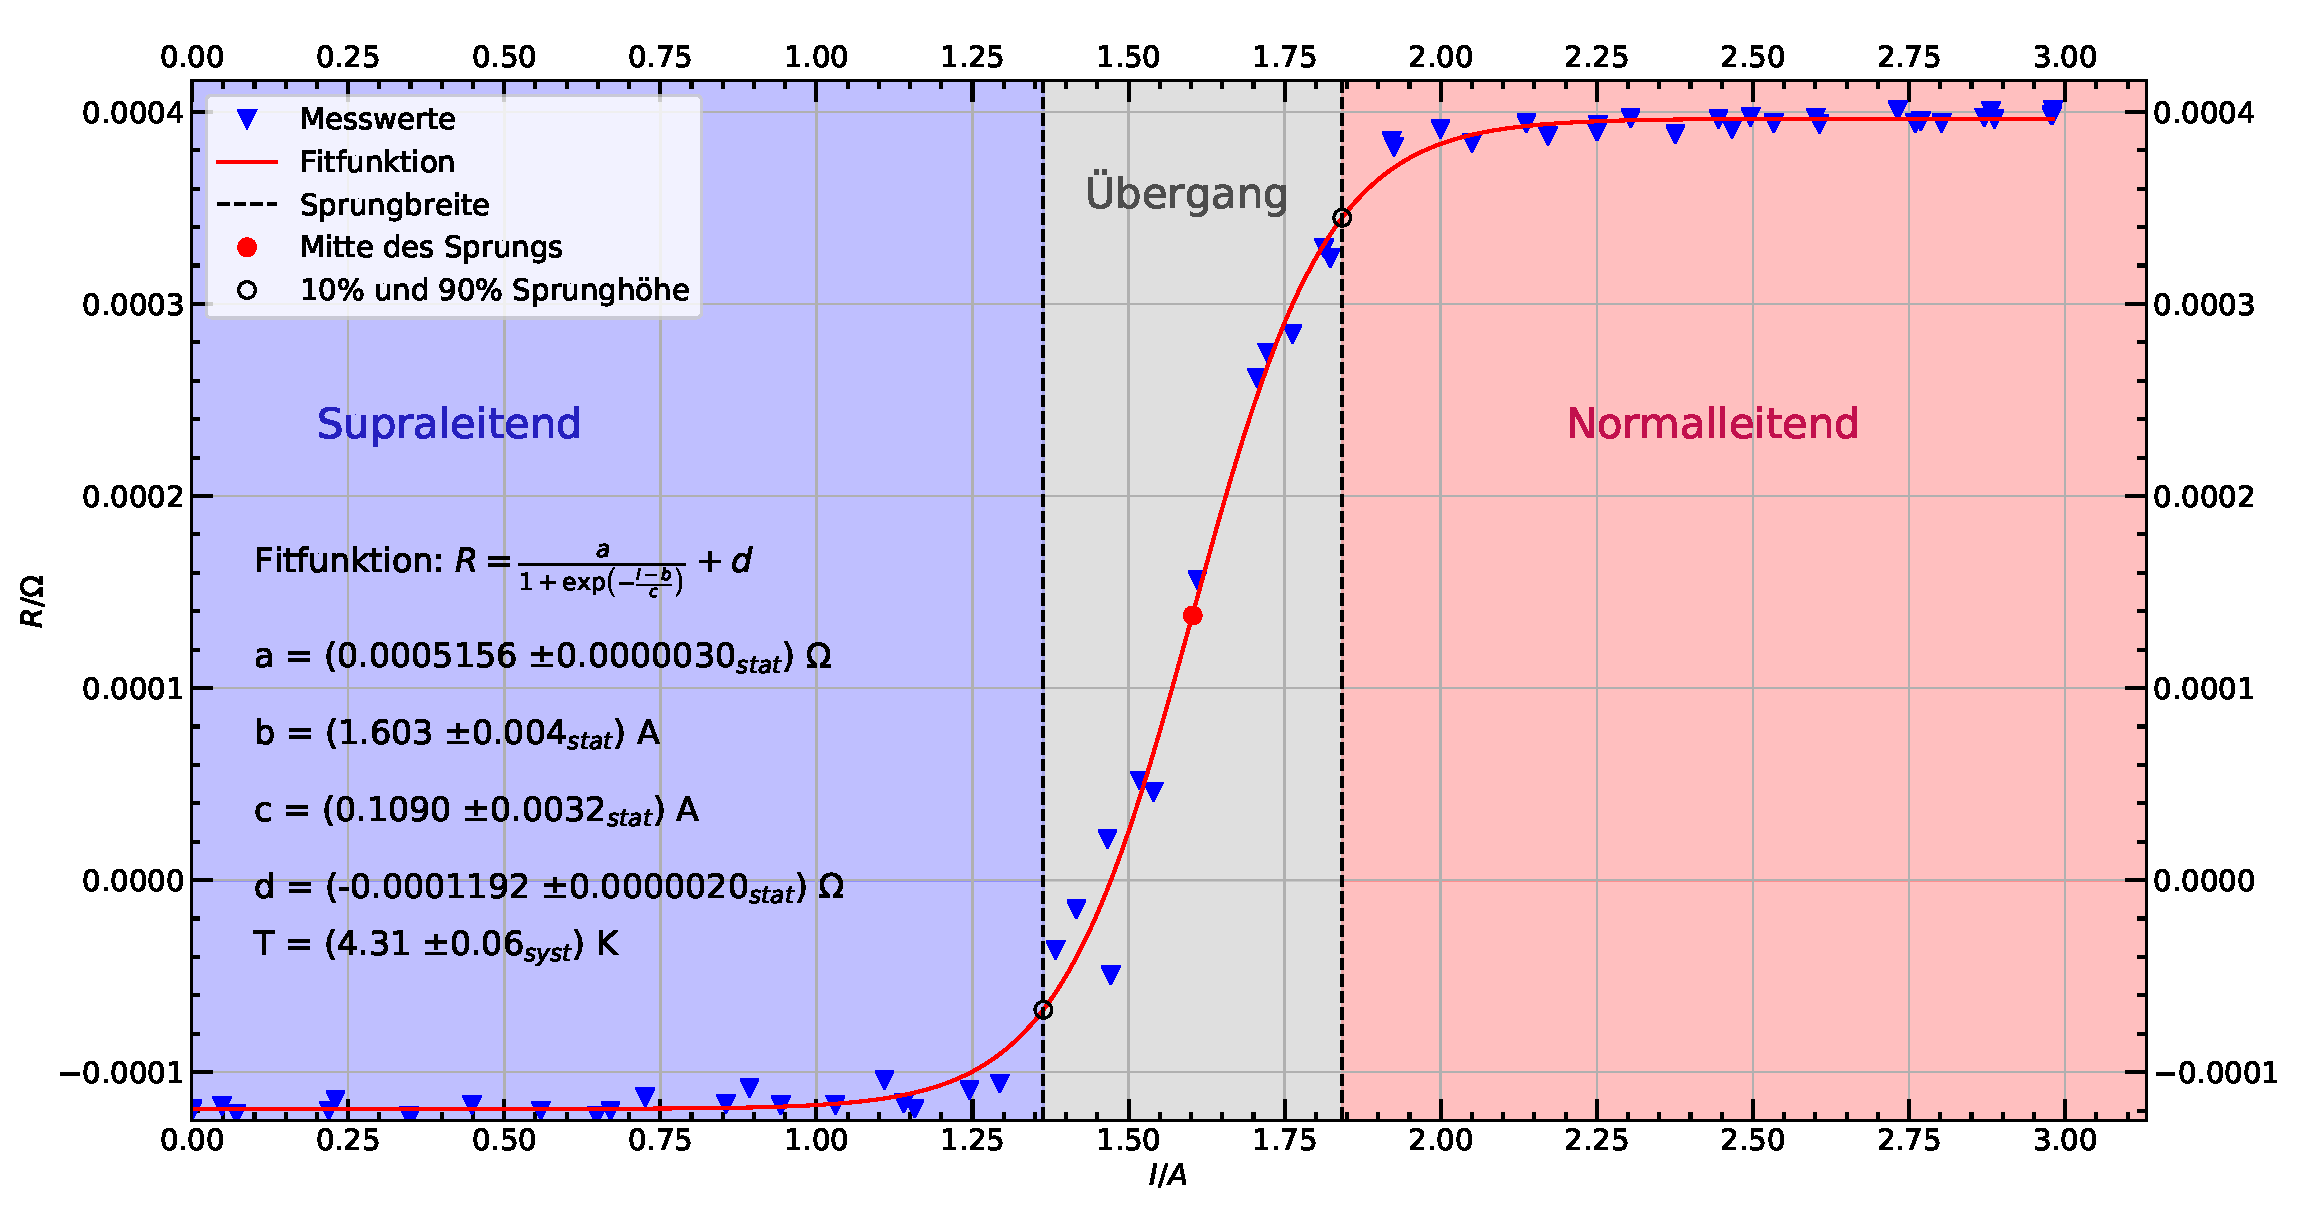
\includegraphics[width=\textwidth]{Fitverfahren}
\caption{Messwerte für T = $4.31$\,K.}
\end{figure}
In der Messung wurde die Spannung in Abhängigkeit vom Spulenstrom $I$ gemessen. Dabei wurde der Strom zur Widerstandsbestimmung so gewählt, dass $1\, \Omega$ gerade $1$\,V entspricht. Im Plot ist deutlich der Sprung des Widerstandes zu erkennen. Dabei sind für diesen teilweise negative Werte eingetragen, was an der Kalibrierung des Messgerätes liegt. Um nun die Stromstärke des kritischen Magnetfeldes zu bestimmen, wurde ein Fit mit der im Plot angegeben Fitfunktion durchgeführt und der Sprung erfolgt gerade bei dem Wert des Fitparameters $b$. 
\\\\
Dies wurde nun für die anderen Temperaturen, wie in der Durchführung beschrieben, durchgeführt.
Die jeweiligen Messbedingungen, also die Temperatur und der Druck sind in Tabelle 1 dargestellt.
\newpage
\begin{table} \centering
\begin{tabular}{|c|c|}
\hline
\(T\)/K & p/mbar \\\hline
4.309 & 1043\\\hline
4.327 & 1043\\\hline
4.351 & 1043\\\hline
4.046 & 787\\\hline
3.883 & 673\\\hline
3.607 & 461\\\hline
3.305 & 318\\\hline
3.160 & 255\\\hline
3.038 & 208\\\hline
2.845 & 145\\\hline
2.586 & 80\\\hline
2.393 & 50\\\hline
2.330 & 44\\\hline
2.058 & 9\\\hline
4.419 & 1019\\\hline
4.599 & 1018\\\hline
4.798 & 1018\\\hline
4.997 & 1019\\\hline
5.194 & 1020\\\hline
5.397 & 1019\\\hline
5.598 & 1018\\\hline
5.798 & 1018\\\hline
5.998 & 1018\\\hline
6.199 & 1018\\\hline
6.399 & 1018\\\hline
6.598 & 1018\\\hline
6.797 & 1019\\\hline
\end{tabular}
\caption{Druck der Messung für verschiedene Temperaturen.}
\label{tab1}
\end{table}
Für die Temperaturen unter $4.2$\,K ist also, wie bereits diskutiert, der Druck deutlich geringer, damit diese überhaupt erreicht werden können. Für die Temperaturen über $4.2$\,K ist der Druck praktisch konstant und zwar gleich dem Umgebungsdruck.
\newpage
Die dann mit der oben beschriebenen Methode bestimmten kritischen Werte, also die kritische Stromstärke, das kritische Magnetfeld und deren Unsicherheiten sind in Tabelle 2 zu finden.
\\
\begin{table} [h!]\centering 
\begin{tabular}{|c|c|c|c|c|c|c|c|}
\hline
\(T\)/K & \(\Delta T_{\mathrm{syst}}\)/ K & \(I_{\mathrm{S}}\)/A & \(\Delta I_{\mathrm{S,syst}}\)/A  & \(\Delta I_{\mathrm{S,stat}}\)/A  & \(B_{\mathrm{S}}\)/Gs & \(\Delta B_{\mathrm{S,syst}}\)/Gs  & \(\Delta B_{\mathrm{S,stat}}\)/Gs \\\hline
2.058 & 0.008 & 2.5965 & 0.2502 & 0.0015 & 763.502 & 73.560 & 0.446\\\hline
2.330 & 0.008 & 2.5009 & 0.2752 & 0.0023 & 735.386 & 80.927 & 0.666\\\hline
2.393 & 0.015 & 2.4783 & 0.2693 & 0.0037 & 728.761 & 79.179 & 1.090\\\hline
2.586 & 0.007 & 2.3996 & 0.2908 & 0.0022 & 705.607 & 85.497 & 0.637\\\hline
2.845 & 0.006 & 2.2882 & 0.2923 & 0.0021 & 672.841 & 85.961 & 0.606\\\hline
3.038 & 0.007 & 2.2034 & 0.3038 & 0.0025 & 647.908 & 89.323 & 0.729\\\hline
3.160 & 0.006 & 2.1465 & 0.2855 & 0.0023 & 631.186 & 83.952 & 0.684\\\hline
3.305 & 0.006 & 2.0767 & 0.2939 & 0.0035 & 610.653 & 86.412 & 1.034\\\hline
3.607 & 0.006 & 1.9327 & 0.2786 & 0.0028 & 568.303 & 81.915 & 0.817\\\hline
3.883 & 0.017 & 1.7995 & 0.2596 & 0.0022 & 529.135 & 76.348 & 0.659\\\hline
4.046 & 0.005 & 1.7573 & 0.2590 & 0.0070 & 516.742 & 76.167 & 2.045\\\hline
4.309 & 0.004 & 1.6028 & 0.2393 & 0.0040 & 471.301 & 70.361 & 1.167\\\hline
4.327 & 0.010 & 1.5501 & 0.2424 & 0.0035 & 455.809 & 71.286 & 1.028\\\hline
4.351 & 0.016 & 1.5579 & 0.2612 & 0.0039 & 458.104 & 76.801 & 1.152\\\hline
4.419 & 0.014 & 1.5489 & 0.2329 & 0.0020 & 455.467 & 68.497 & 0.576\\\hline
4.599 & 0.005 & 1.4573 & 0.2266 & 0.0030 & 428.514 & 66.647 & 0.875\\\hline
4.798 & 0.002 & 1.3636 & 0.2137 & 0.0052 & 400.977 & 62.851 & 1.541\\\hline
4.997 & 0.002 & 1.2269 & 0.1955 & 0.0026 & 360.781 & 57.496 & 0.761\\\hline
5.194 & 0.004 & 1.1152 & 0.1990 & 0.0018 & 327.930 & 58.522 & 0.521\\\hline
5.397 & 0.002 & 0.9906 & 0.1897 & 0.0019 & 291.292 & 55.778 & 0.564\\\hline
5.598 & 0.003 & 0.8701 & 0.1528 & 0.0013 & 255.844 & 44.920 & 0.387\\\hline
5.798 & 0.002 & 0.7403 & 0.1466 & 0.0011 & 217.674 & 43.113 & 0.329\\\hline
5.998 & 0.002 & 0.6064 & 0.1286 & 0.0008 & 178.308 & 37.813 & 0.246\\\hline
6.199 & 0.002 & 0.4549 & 0.1135 & 0.0029 & 133.778 & 33.379 & 0.857\\\hline
6.399 & 0.002 & 0.3240 & 0.0909 & 0.0010 & 95.261 & 26.734 & 0.284\\\hline
6.598 & 0.001 & 0.1733 & 0.0918 & 0.0020 & 50.960 & 26.994 & 0.578\\\hline
6.797 & 0.002 & 0.0326 & 0.0721 & 0.0057 & 9.571 & 21.188 & 1.676\\\hline
\end{tabular}
\caption{Kritische Werte der magnetischen Flussdichte \(B\) in Abhängigkeit von der Temperatur \(T\) für Blei.}
\label{t} 
\end{table}
\newpage
Es war bereits während der Durchführung des Versuchs deutlich zu beobachten, dass die kritische Stromstärke für eine zunehmende Temperatur immer kleiner wurde. Dies ist nochmals in Abbildung 9 illustriert.
\\\\
\begin{figure}[h!]
\centering
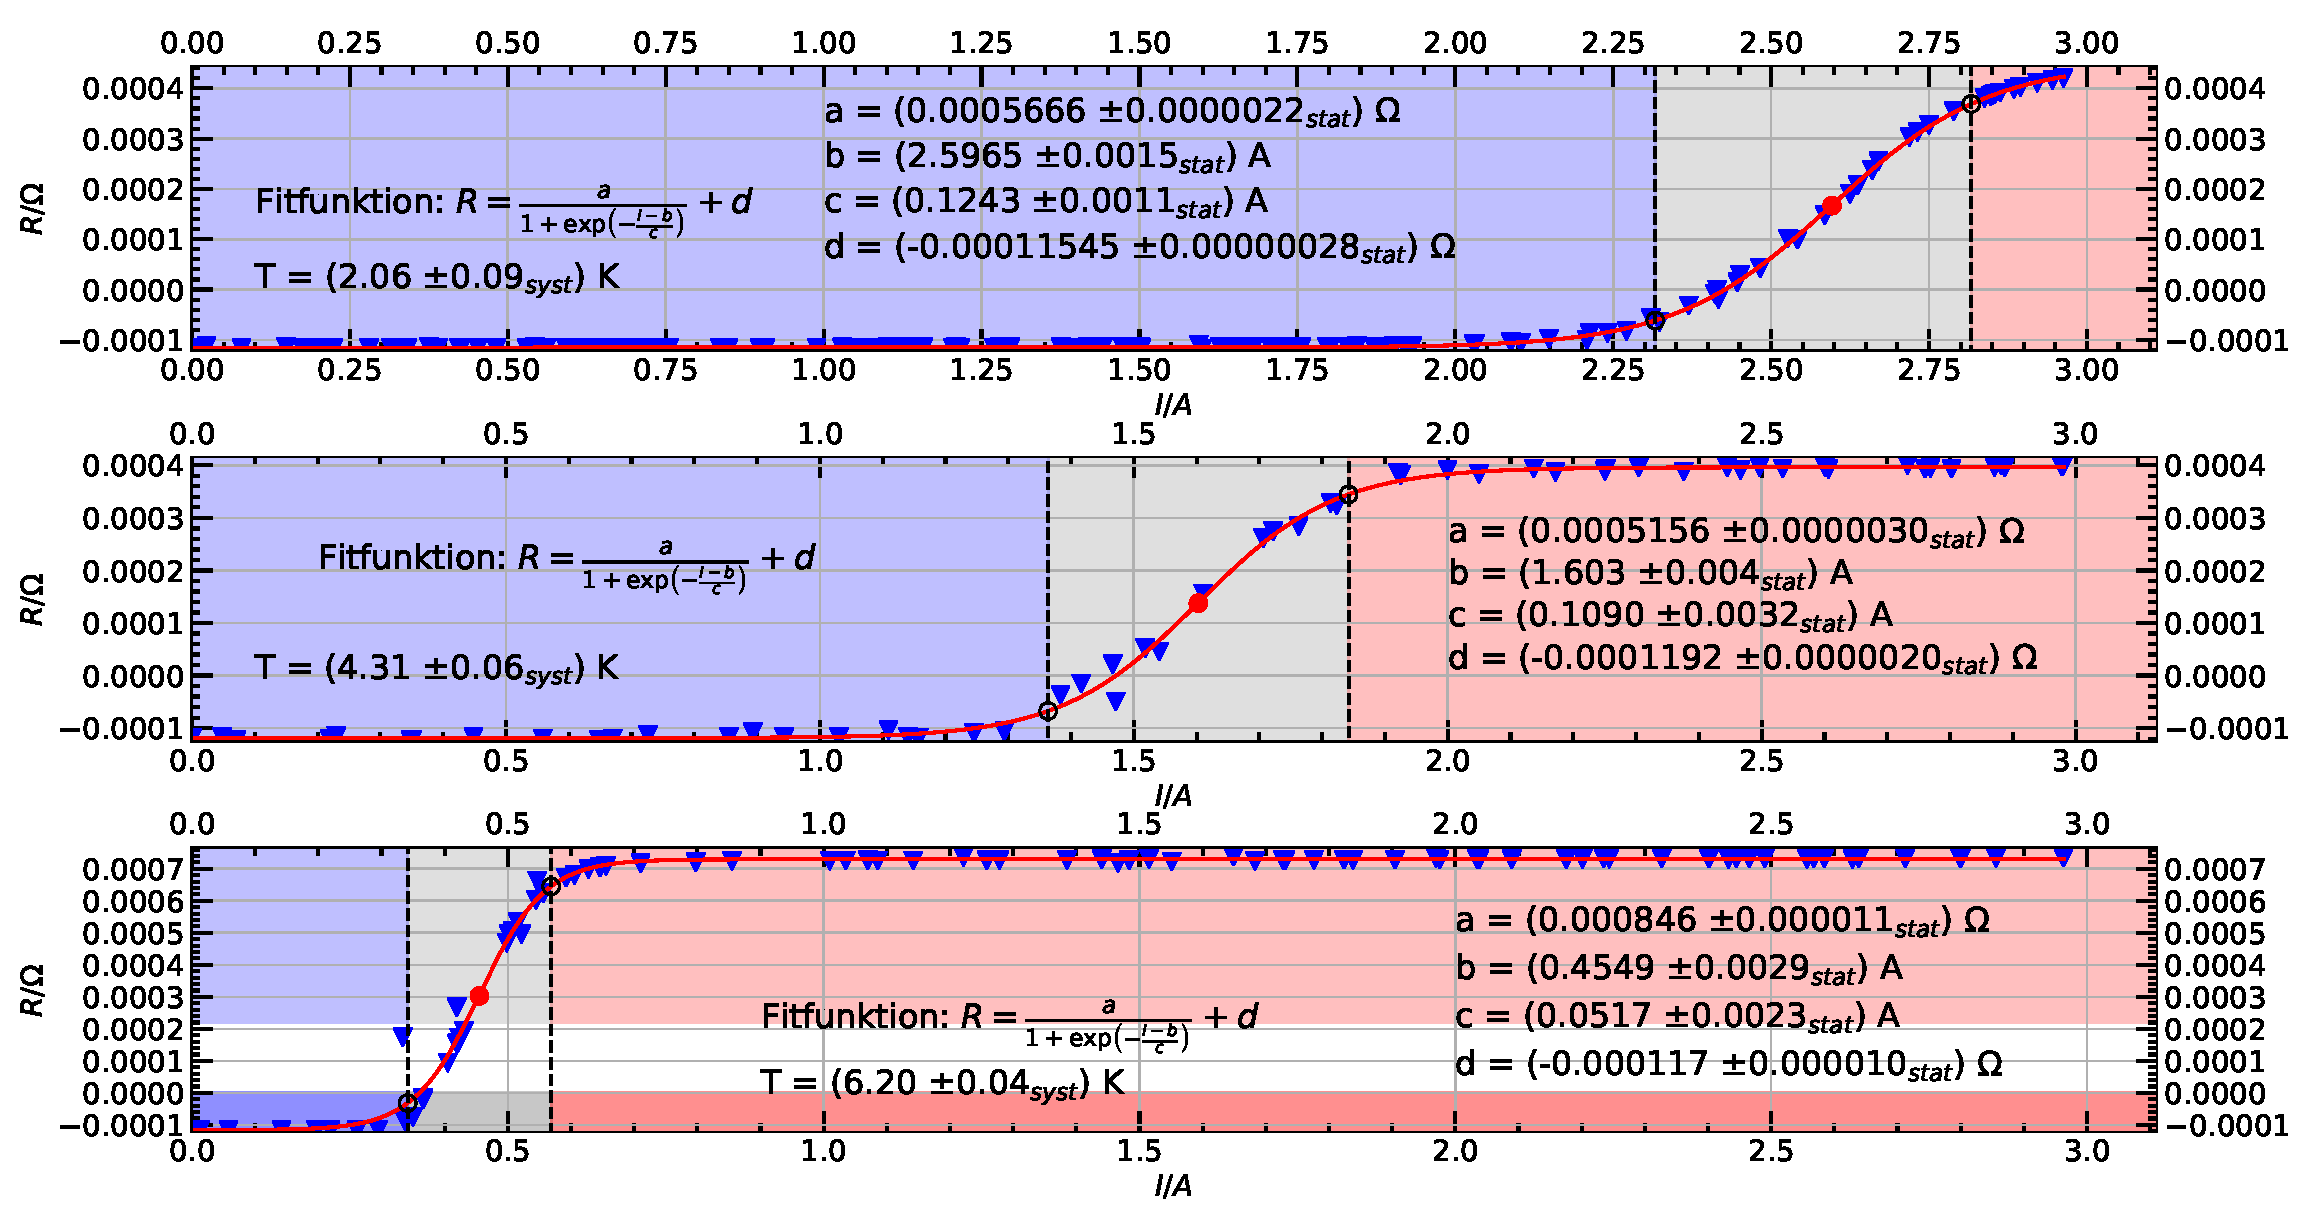
\includegraphics[width=\textwidth]{verschiedene_Temperaturen}
\caption{Darstellung der Messwerte für 3 verschiedene Temperaturen.}
\end{figure}
\\\\
Der Sprung erfolgte also immer früher, bis er bei einer Temperatur von $6.797$\,K praktisch gar nicht mehr erfolgte, sodass die Aufnahme der Messwerte bei dieser Temperatur beendet werden konnte, da die Probe bei dieser Temperatur die ganze Zeit normalleitend war (Abbildung 10).
\\\\
\begin{figure}[h!]
\centering
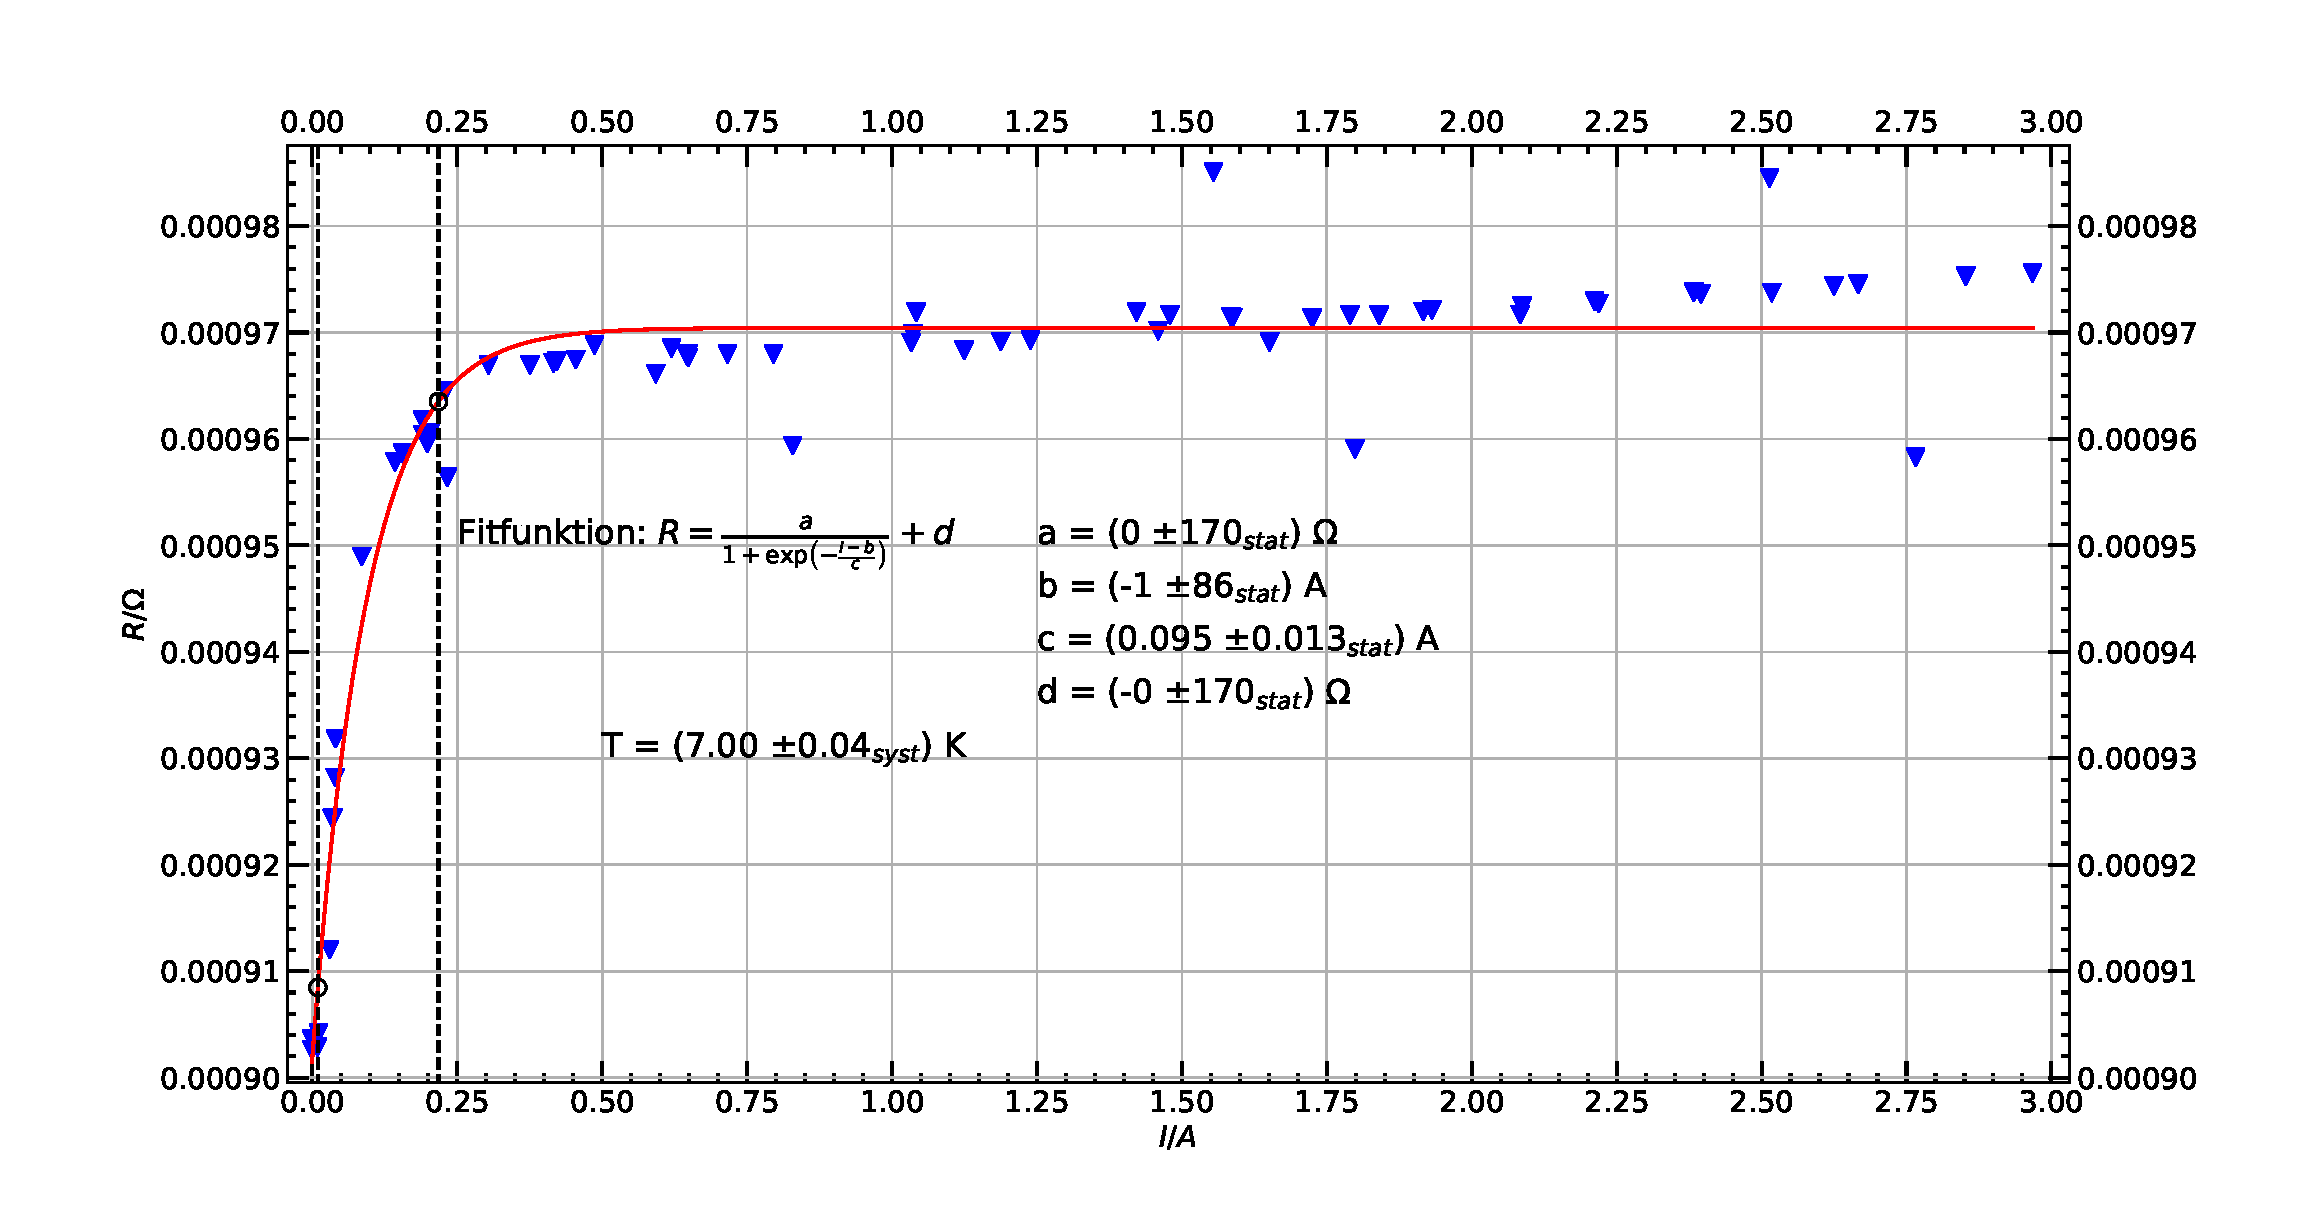
\includegraphics[width=\textwidth]{letzte_Messung.pdf}
\caption{Letzte Messung, bei T = $6.797$\,K.}
\end{figure}
\newpage
\subsection{Bestimmung der Parameter $\text{H}_{\text{C,0}}$ und $\text{T}_{\text {C}}$ und Vergleich mit der Literatur}
Die Werte aus Tabelle (\ref{t}) können nun in einem Phasendiagramm dargestellt werden und nach Gleichung (\ref{h}) gefittet werden (siehe Abbildung 11).
\begin{figure}[h!]
\centering
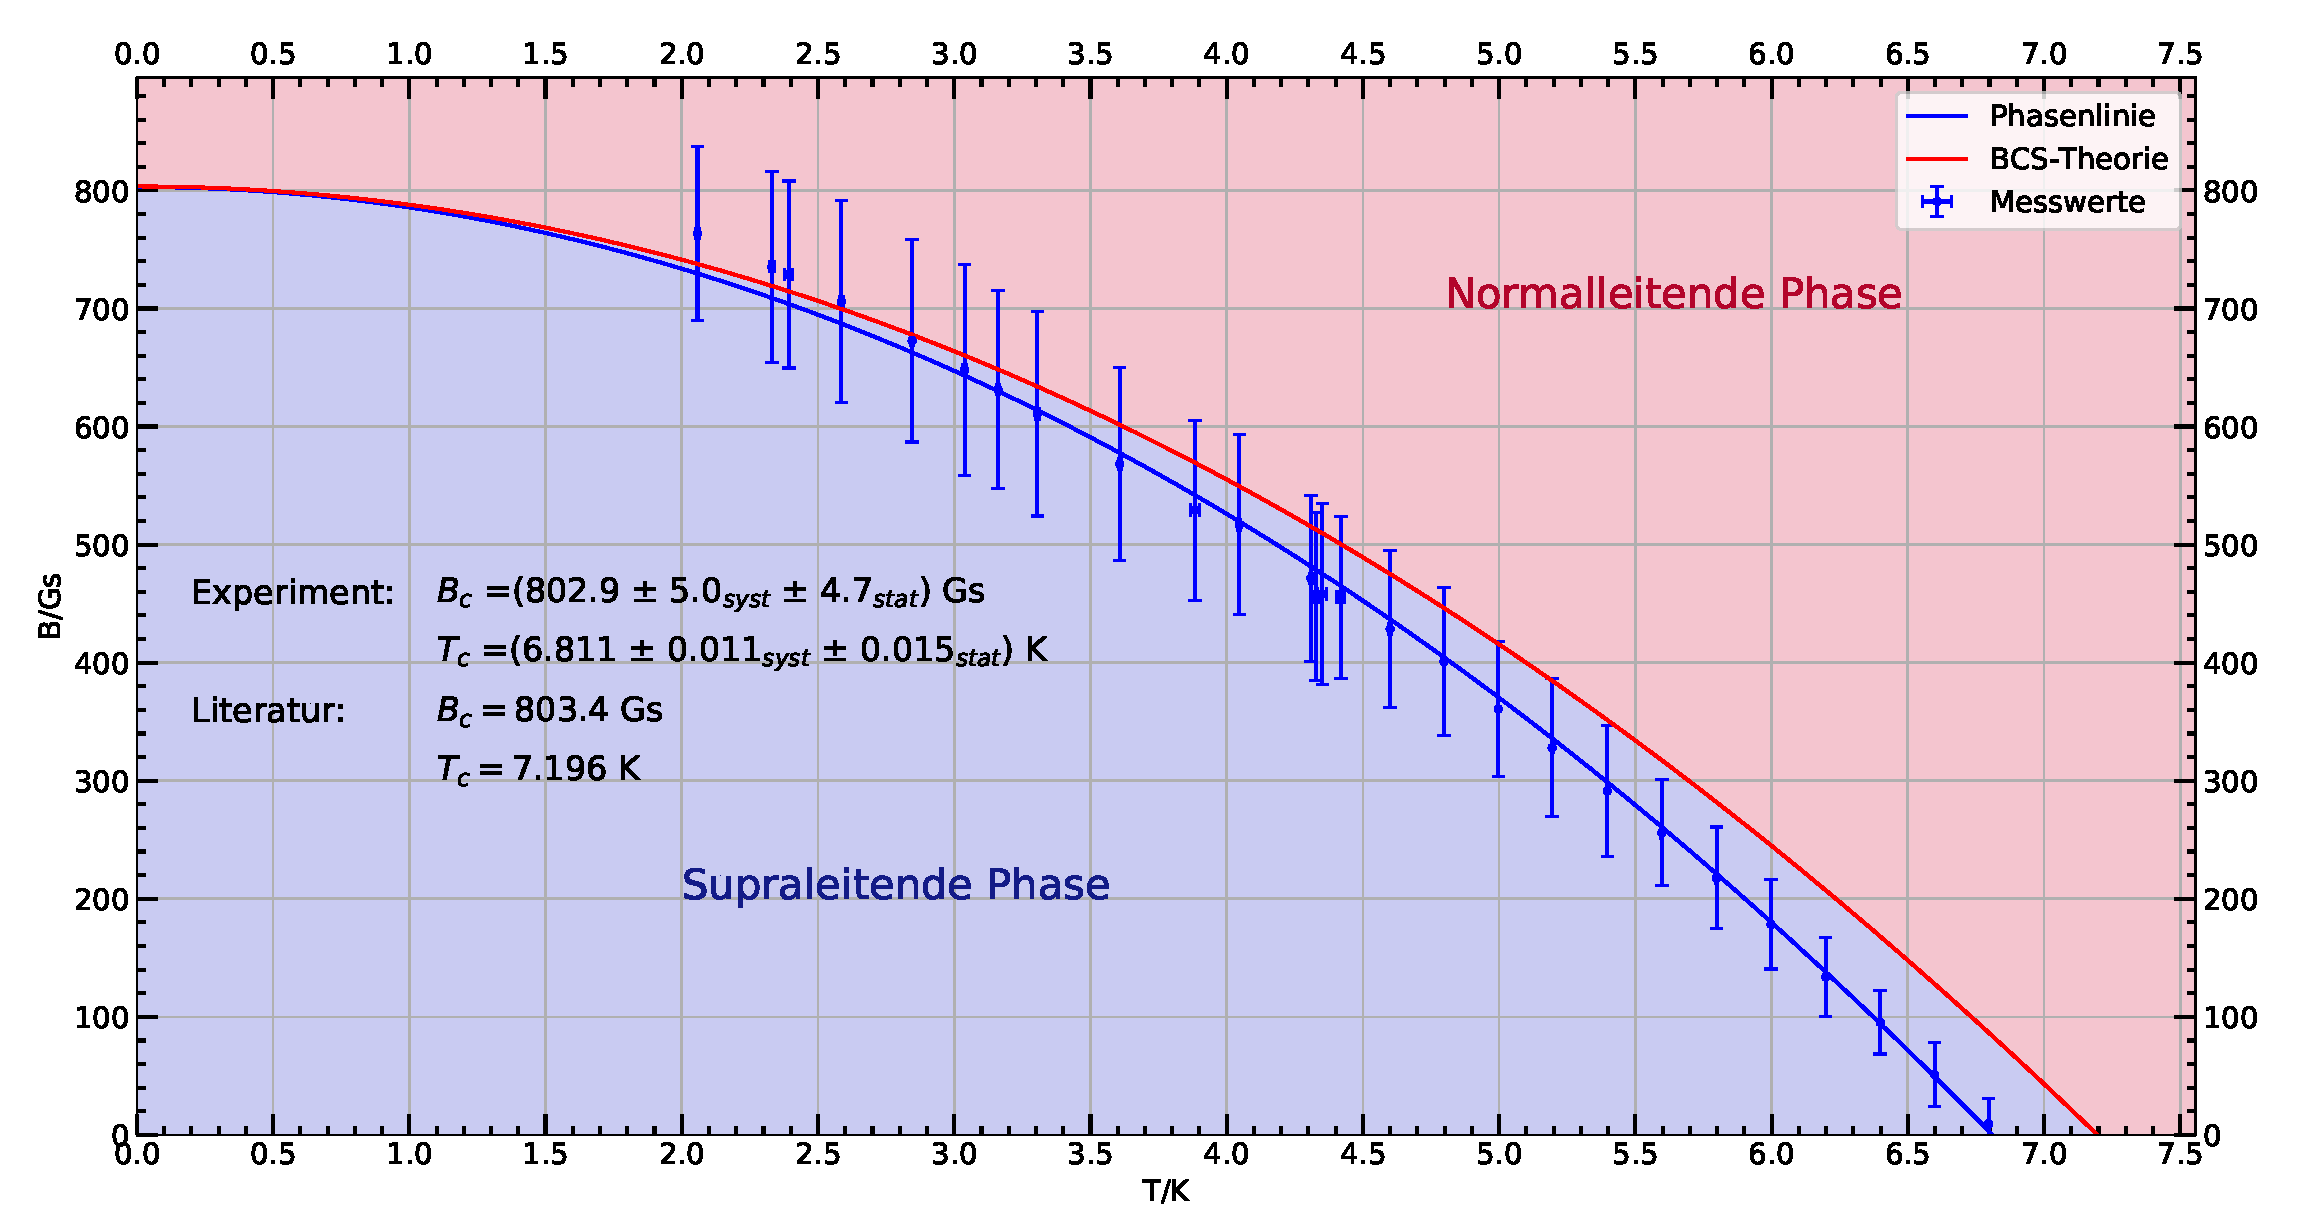
\includegraphics[width=0.835\textwidth]{Phasendiagramm_Blei.pdf}
\caption{Phasendiagramm der Bleiprobe, kritisches Magnetfeld in Abhängigkeit von der Temperatur.}
\end{figure}
\newpage
Die hier verwendeten Theoriewerte (rote Linie) stammen aus \cite{6}. Der prinzipielle Verlauf beider Kurven ist gleich, besonders im Temperaturbereich von $2.0$\,K bis $5.0$\,K stimmen die Messwerte im Rahmen der Messungenauigkeit mit den Literaturwerten überein. Selbiges gilt auch für den durch Fit bestimmten Schnittpunkt mit der y-Achse. Die kritische Temperatur stimmt im Rahmen der Messunsicherheiten nicht mit dem Literaturwert von $7.196$\,K überein. Der Grund dafür muss in einer systematischen Unsicherheit liegen, da die gemessene Kurve unter der Theoriekurve liegt, die Abweichung hat also keinen zufälligen Charakter.
\\\\
Die Abweichung lässt sich dadurch begründen, dass nicht nur die Probe allein, sondern der gesamte Probenraum geheizt werden muss. Dadurch kommt es konstruktionsbedingt stets zu unerwünschten thermischen Verlusten. Andererseits besitzt die Probe eine endliche Ausdehnung und kann nicht instantan homogen temperiert werden. Bei tiefen Temperaturen geht die Wärmekapazität gegen $0$, sodass sich Temperaturunterschiede leichter ausbreiten können, als im Hochtemperaturbereich.

\subsection{Fit für das Ge-Thermometer}
In diesem Teil der Auswertung soll die Kalibrierung des Germanium-Thermometers untersucht werden. Für eine alte Kalibrierkurve sind die Werte aus Abbildung 12 vorgegeben gewesen.
\\
\begin{figure}[h!]
\centering
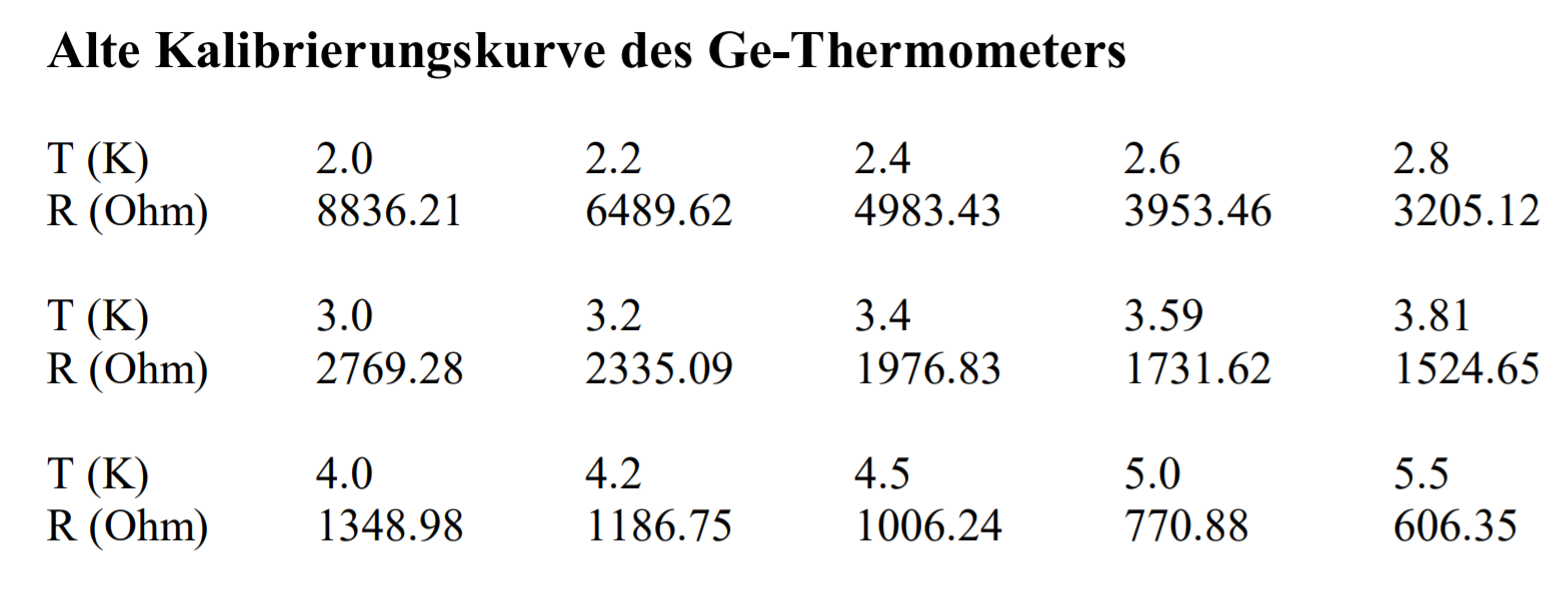
\includegraphics[width=\textwidth]{werte_ge_alt}
\caption{Wertetabelle der alten Kalibrierungskurve des Ge-Thermometers, entnommen aus \cite{3}.}
\end{figure}
\newpage
Ein Fit der Werte ergab Abbildung 13.
\\
\begin{figure}[h!]
\centering
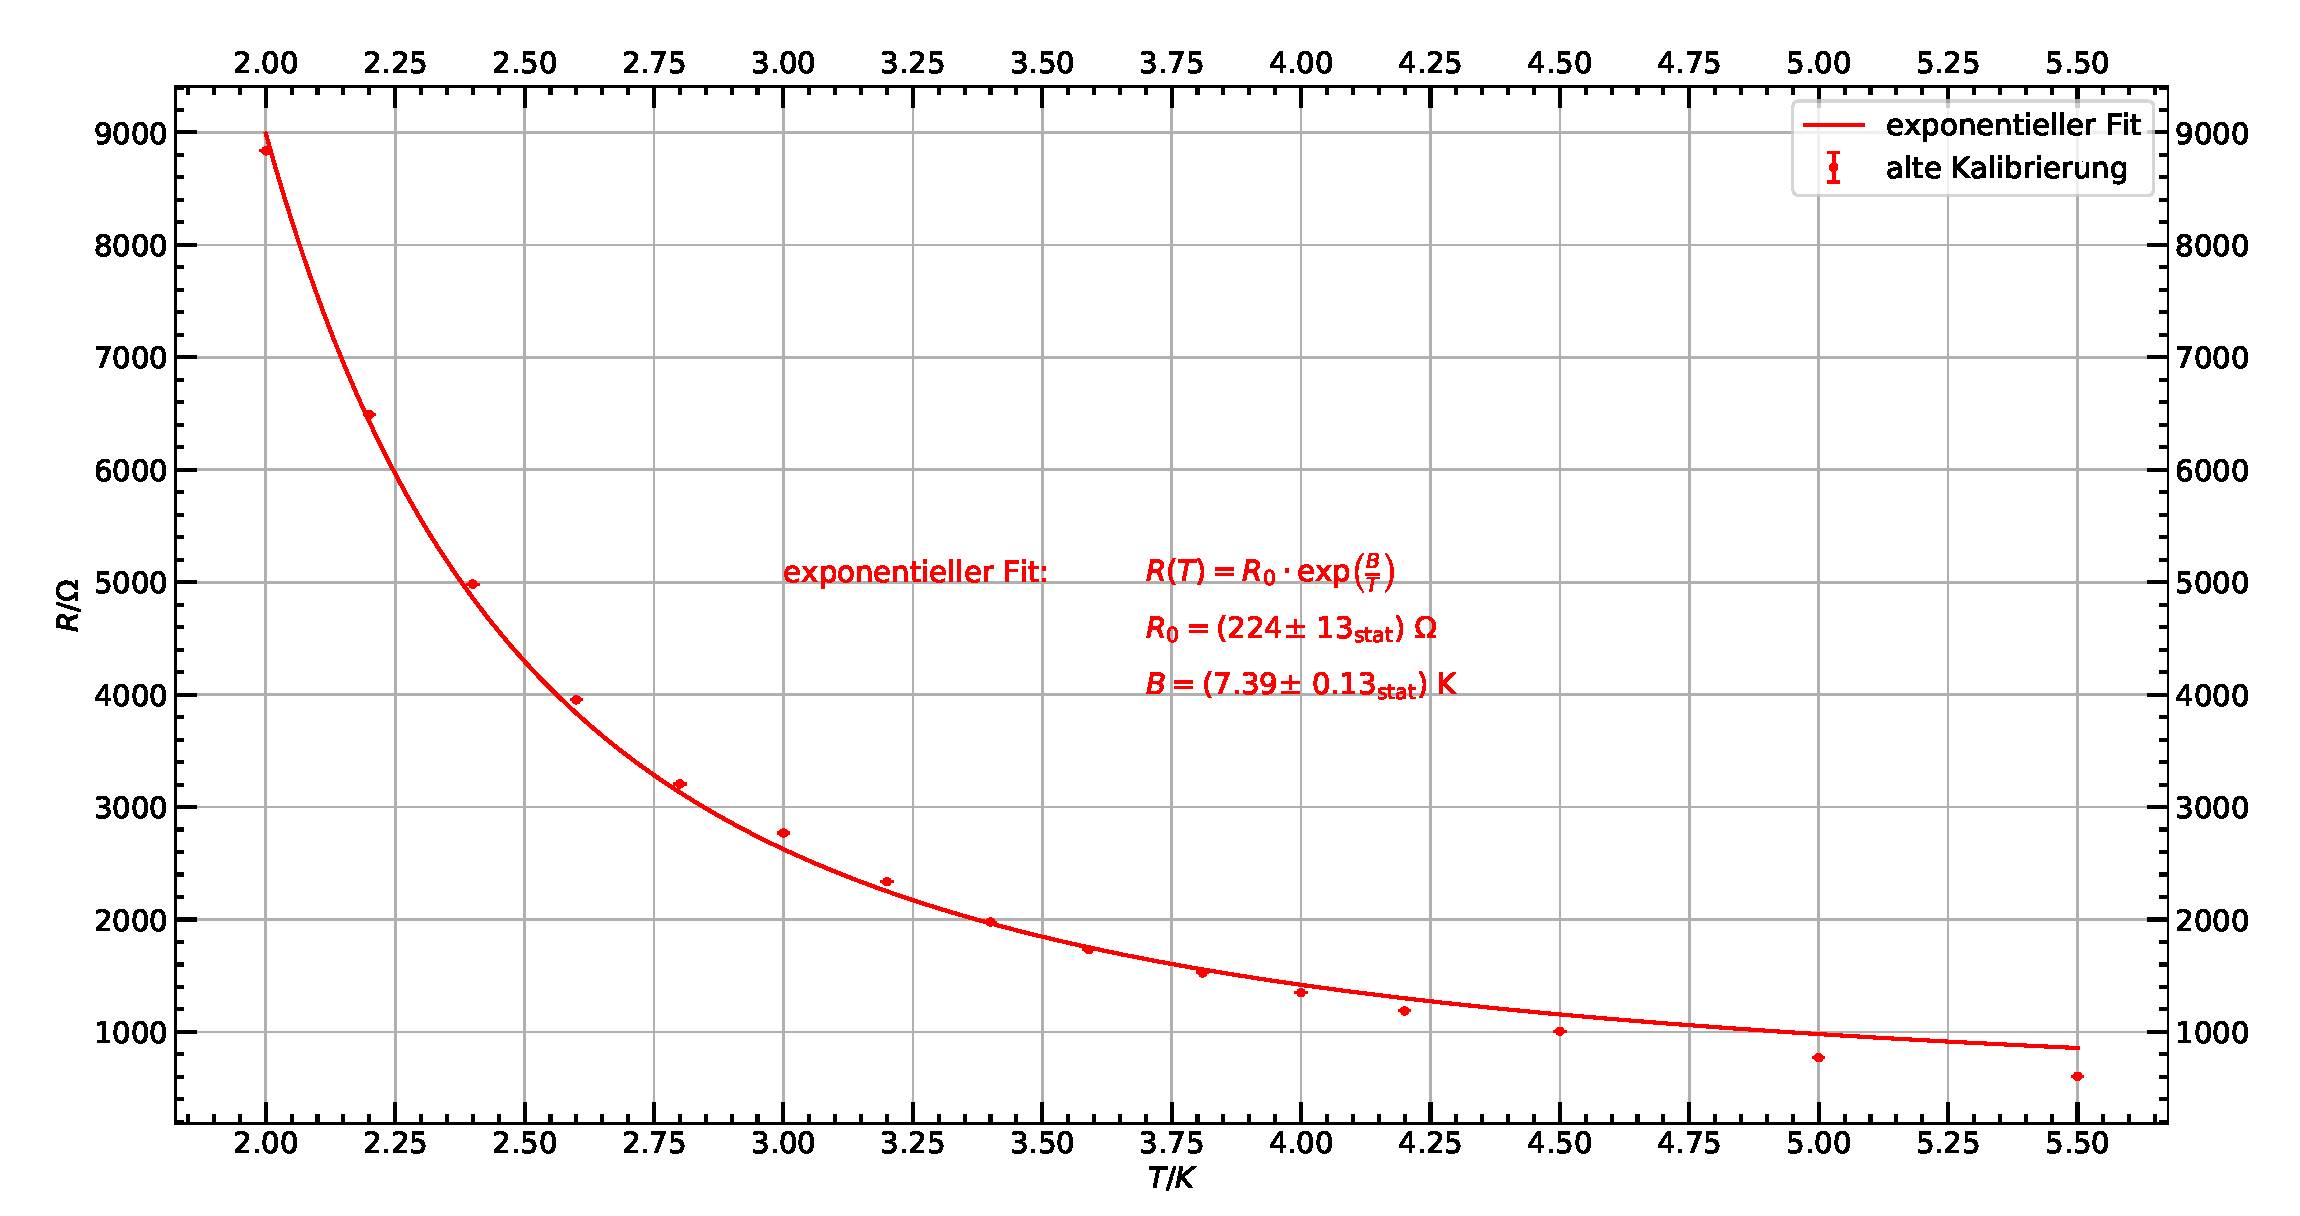
\includegraphics[width=\textwidth]{Ge_Thermometer_alte_Kalibrierung.pdf}
\caption{Fit der alten Kalibrierungskurve des Ge-Thermometers.}
\end{figure}
\\
Die Fitfunktion ist in der Grafik angegeben. Es wurde ein exponentieller Fit verwendet, da es sich um einen Heißleiter handelt. Ein Heißleiter ist durch einen negativen Temperaturkoeffizienten gekennzeichnet. Er leitet den Strom bei höheren Temperaturen deshalb besser und bei tieferen Temperaturen wird der Widerstand größer.
\subsection{Dampfdruckkurve für Helium}
Zudem waren die Werte der Dampfdruckkurve für Helium in Abbildung 14 gegeben.
\newpage
\begin{figure}[h!]
\centering
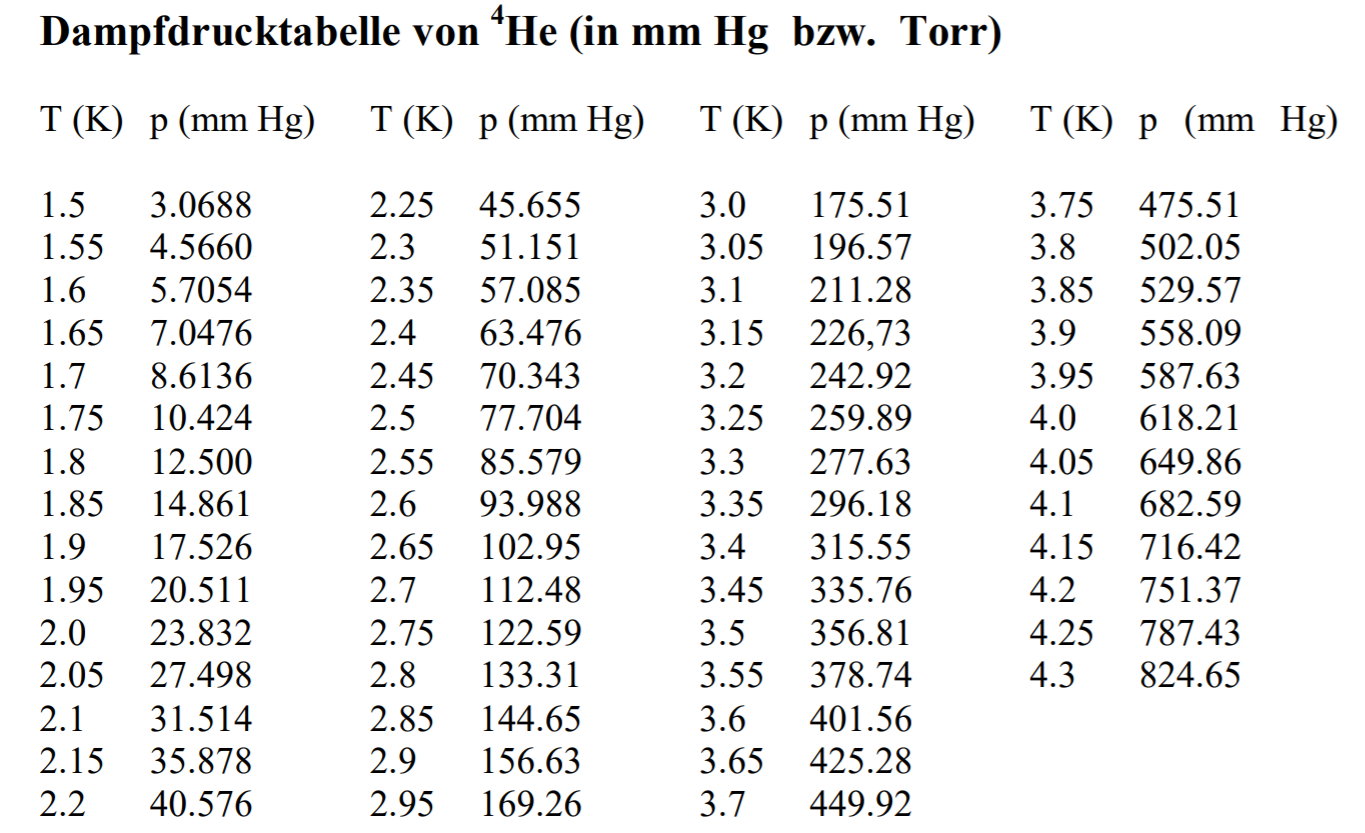
\includegraphics[width=\textwidth]{dampf_werte}
\caption{Werte der Dampfdruckkurve für Helium.}
\end{figure}
Diese erfüllen die Clausius-Clapeyron-Gleichung:
\begin{align}
p(T)= R_0 \cdot e^{\frac{\Delta H_{m,V}}{R\cdot T}}.
\end{align}
Hierbei wird $\Delta H_{m,V}$ im betrachteten Temperaturintervall als Konstant angenommen. Ein Fit mit $p_0$ und $\Delta H_{m,V}$ als freie Parameter ergibt Abbildung 15.
\begin{figure}[h!]
\centering
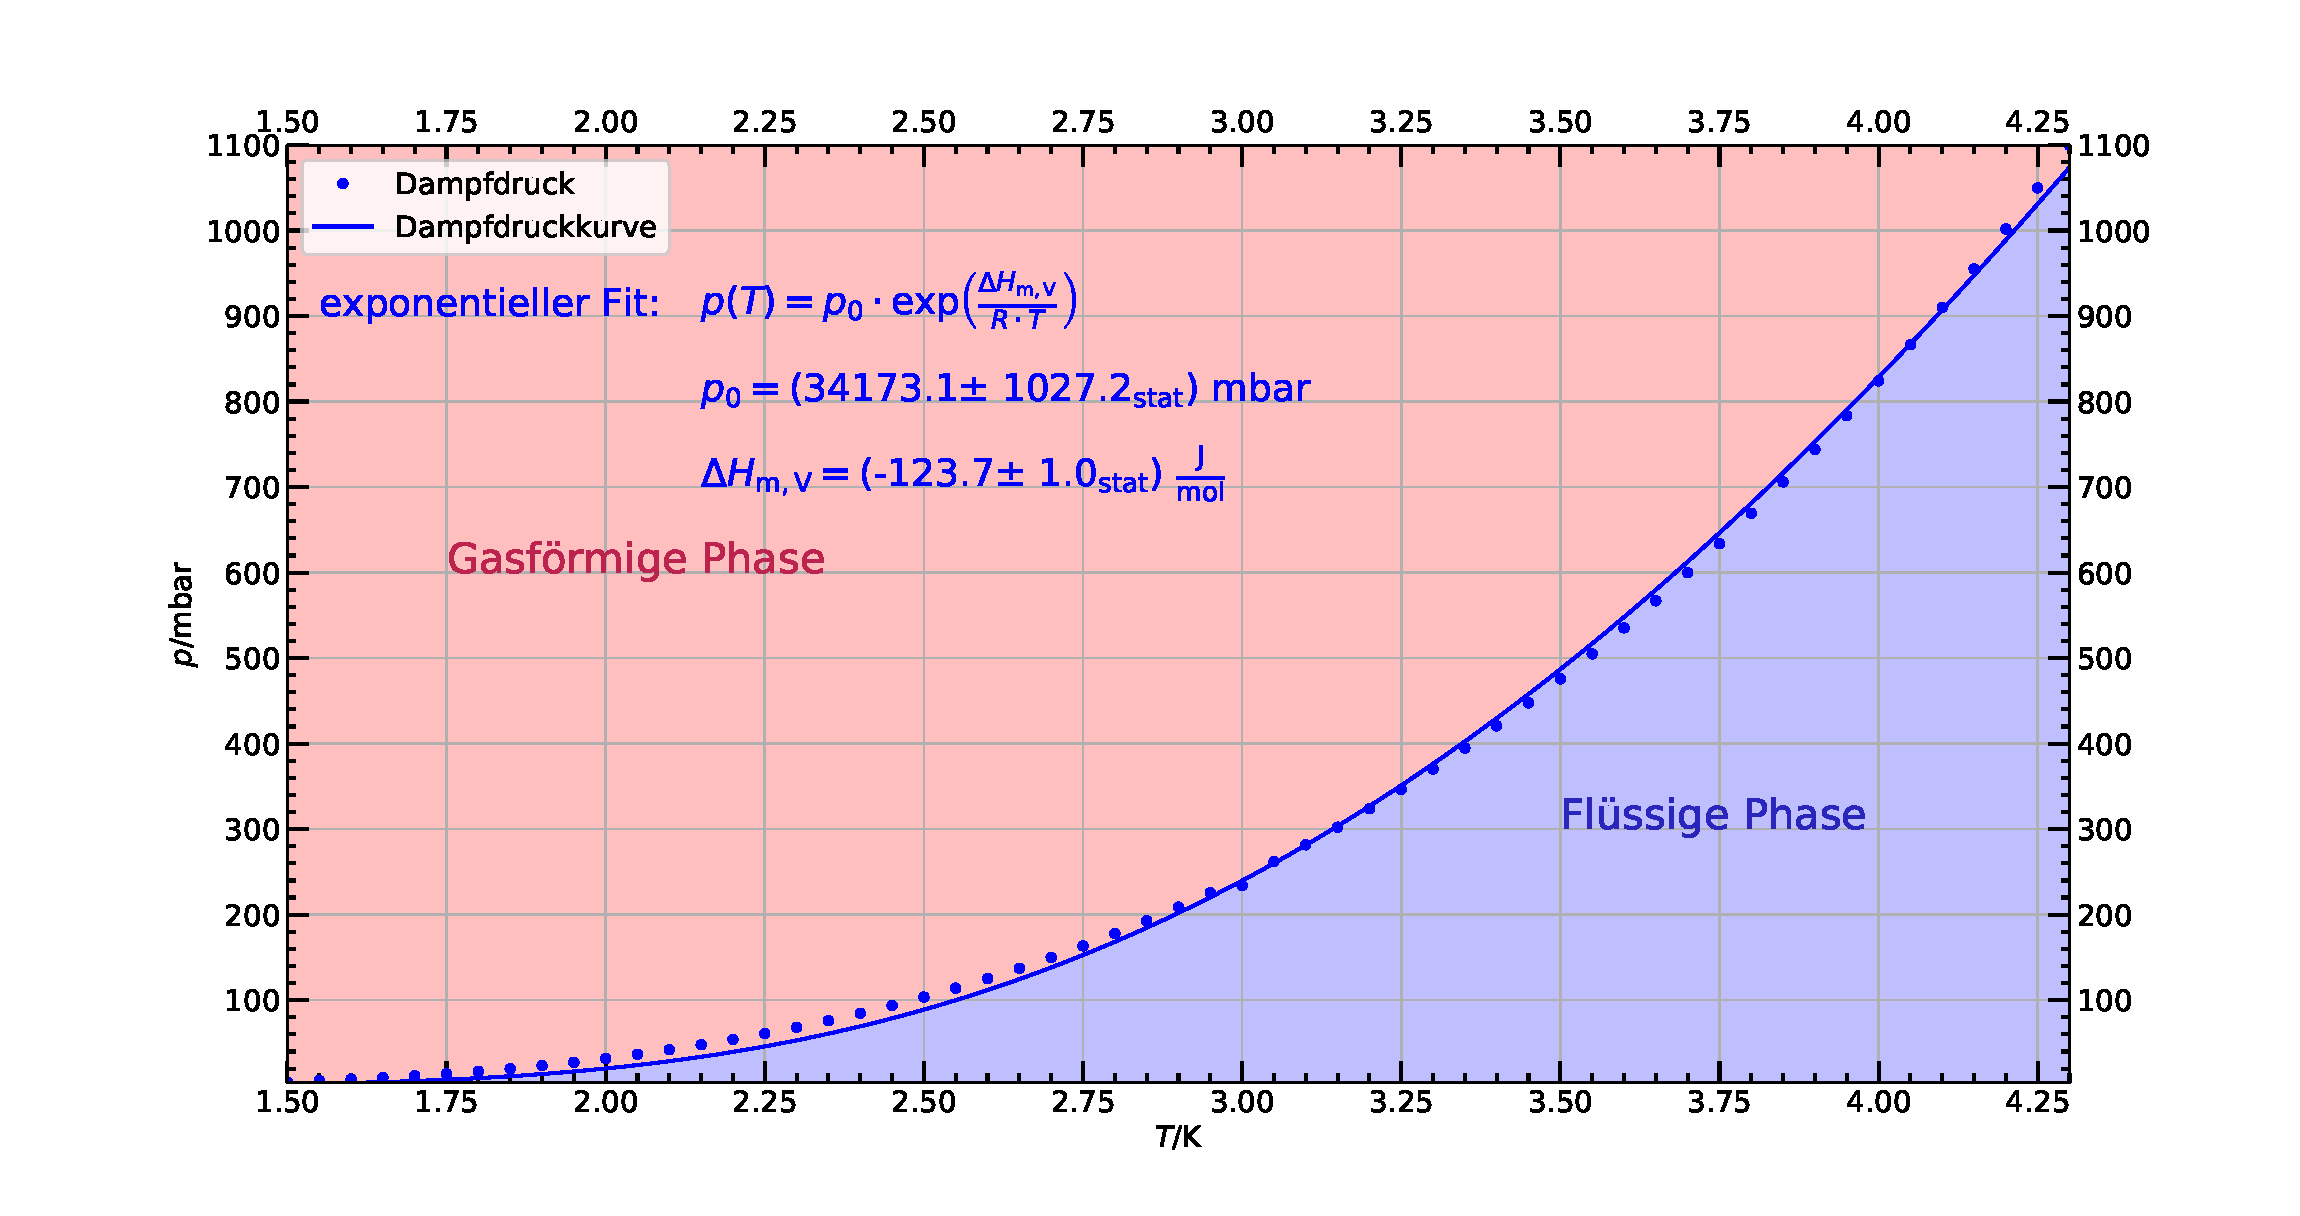
\includegraphics[width=0.8\textwidth]{Dampfdruckkurve_He4.pdf}
\caption{Dampfdruckkurve für Helium.}
\end{figure}
\newpage

\section{Vergleich der Thermometer}
\subsection{Dampfdruckmessung}
Nun kann einerseits mithilfe der Dampfdruckkurve aus den Druckwerten in Tabelle (\ref{tab1}) die Temperatur bestimmt werden. Die so bestimmten Temperaturen werden im Folgenden mit $\text{T}_{\text{Dampf}}$ bezeichnet. Andererseits kann aus dem exponentiellen Fit für das Germanium zu dem jeweilig gemessenen Widerstand ebenfalls eine Temperatur bestimmt werden. Diese wird $\text{T}_{\mathrm{fit}}$ genannt. Nun kann die Differenz $\text{T}_{\mathrm{fit}} - \text{T}_{\text{Dampf}}$ graphisch über $\text{T}_{\text{Dampf}}$ dargestellt werden (Abbildung 16). \\\\
\begin{figure}[h!]\centering
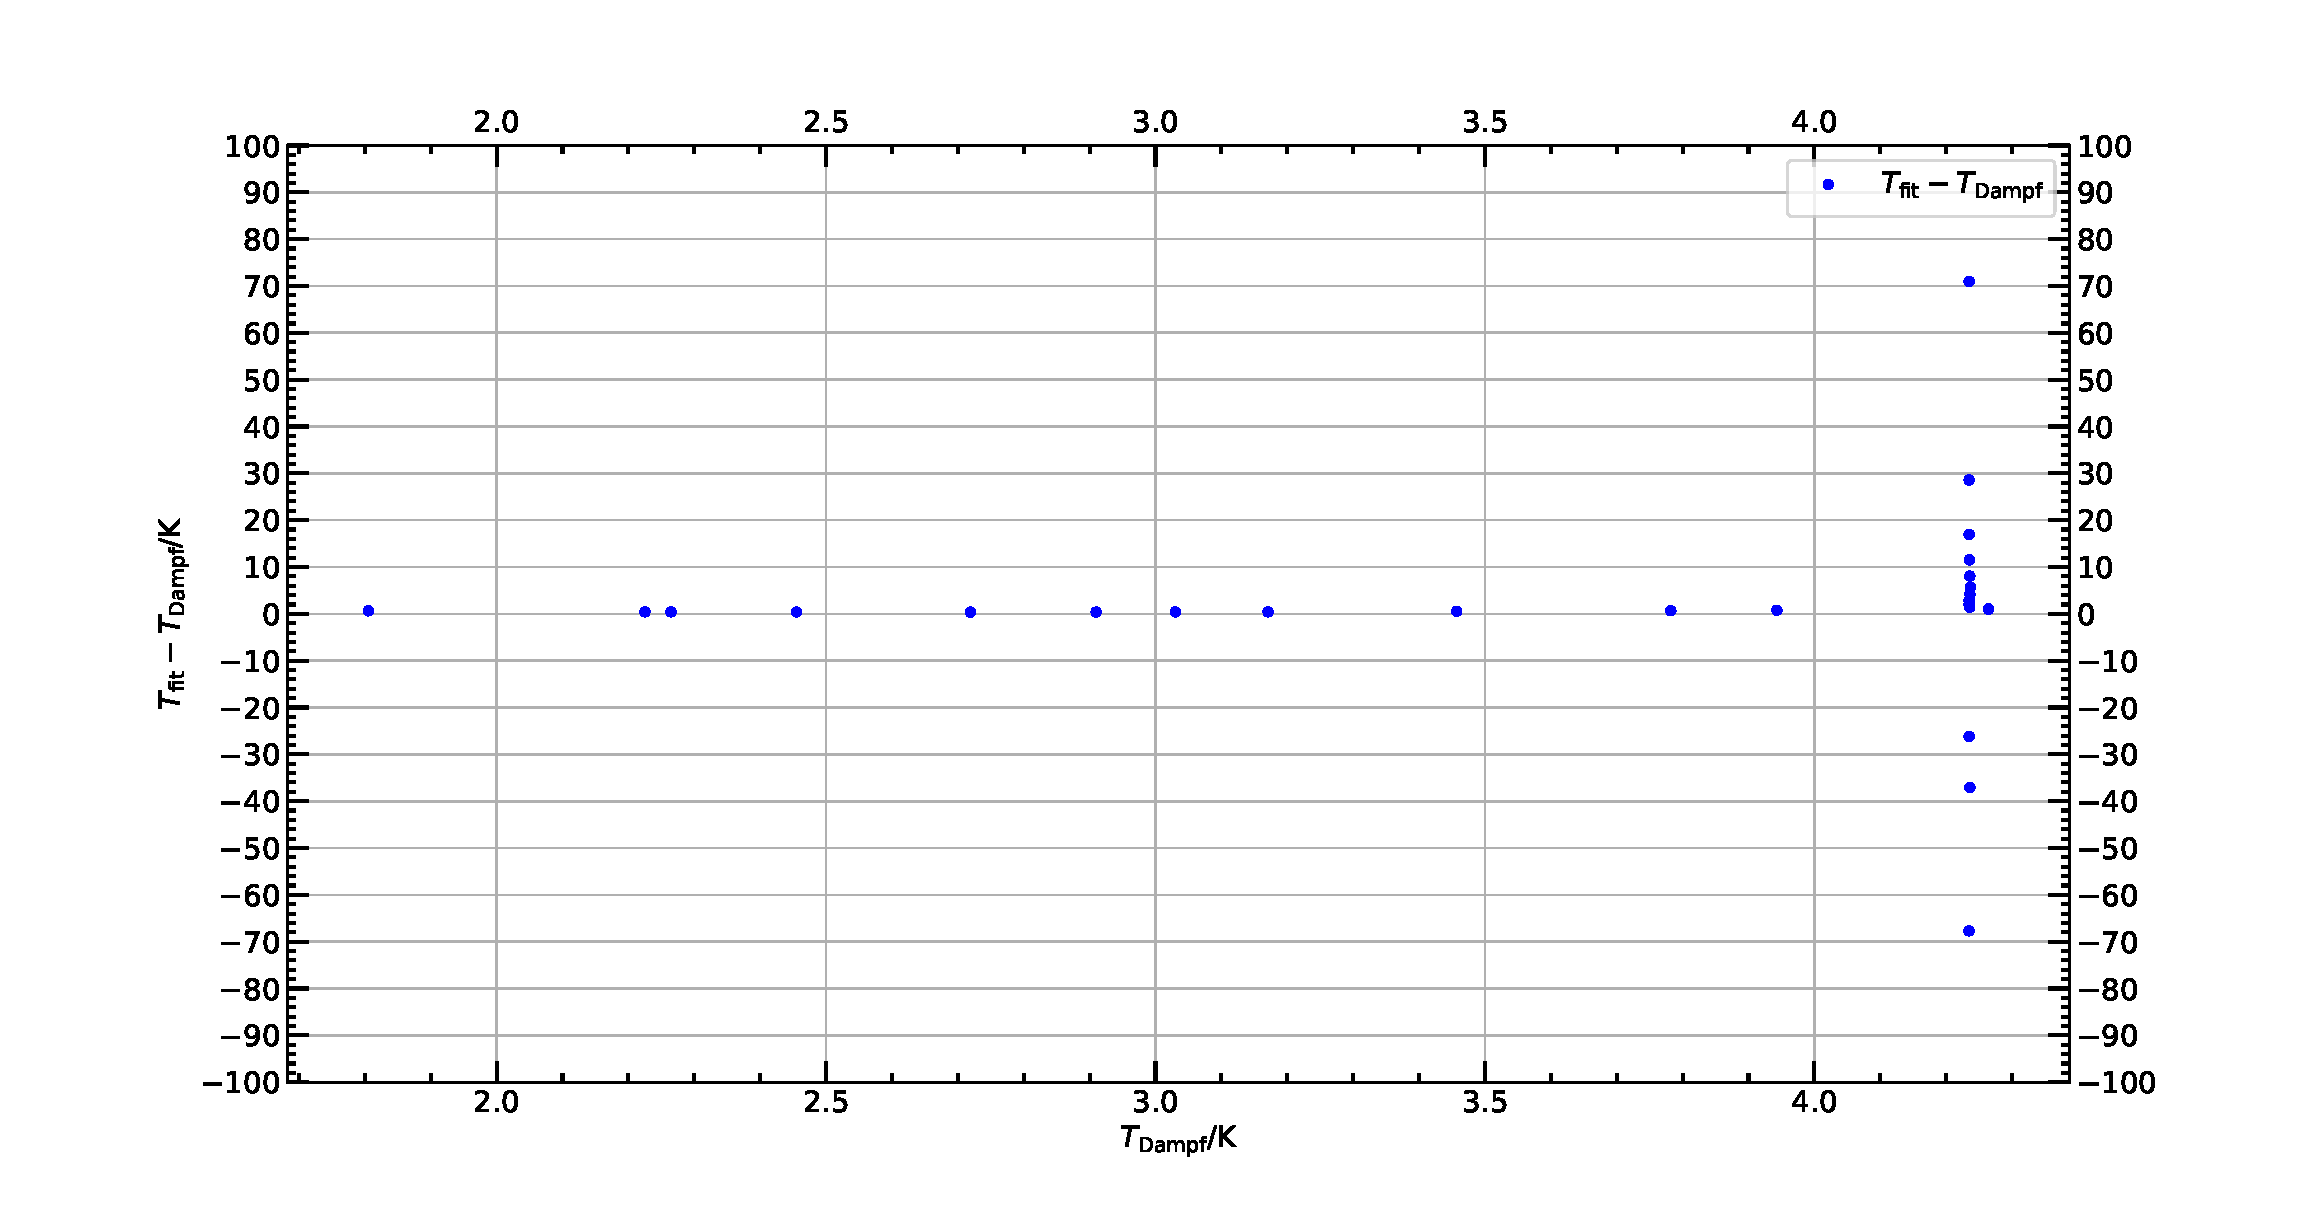
\includegraphics[width=\textwidth]{Germanium_vs_Dampf.pdf}
\caption{Darstellung von $\text{T}_{\mathrm{fit}} - \text{T}_{\text{Dampf}}$ über $\text{T}_{\text{Dampf}}$.}
\end{figure}


Bis zur Siedetemperatur von Helium bei ca. \(T= 4.2 \,\mathrm{K}\) stimmen die Temperaturen des Germaniumthermometers mit denen aus der Dampfdruckkurve bestimmten sehr gut überein, sodass deren Differenz nahe bei null liegt. Bei \(T= 4.2 \,\mathrm{K}\) siedet Helium, sodass dessen Temperatur dort konstant bleibt, obwohl sich die Probenkammer erwärmen kann. Deswegen versagt die Bestimmung der Temperatur über den Dampfdruck an dieser Stelle und es kommt zu einer deutlichen Abweichung vom Wert des Germaniumthermometers.
\subsection{Germaniumthermometer}
Um die Qualität des durchgeführten Fits für das Germaniumthermometer zu überprüfen, wurde die Fitfunktion auf die Widerstandswerte der alten Eichpunkte angewendet. Dies ergibt Temperaturwerte \(T_{\mathrm{fit}}\), die man mit den entsprechenden Werten \(T_{\mathrm{alt}}\) aus der alten Eichtabelle vergleichen kann. Hierfür bietet es sich an, die Differenz \(T_{\mathrm{fit}}- T_{\mathrm{alt}}\) über \(T_{\mathrm{fit}}\) darzustellen (Abbildung 17). \\\\
\begin{figure}[h!]\centering
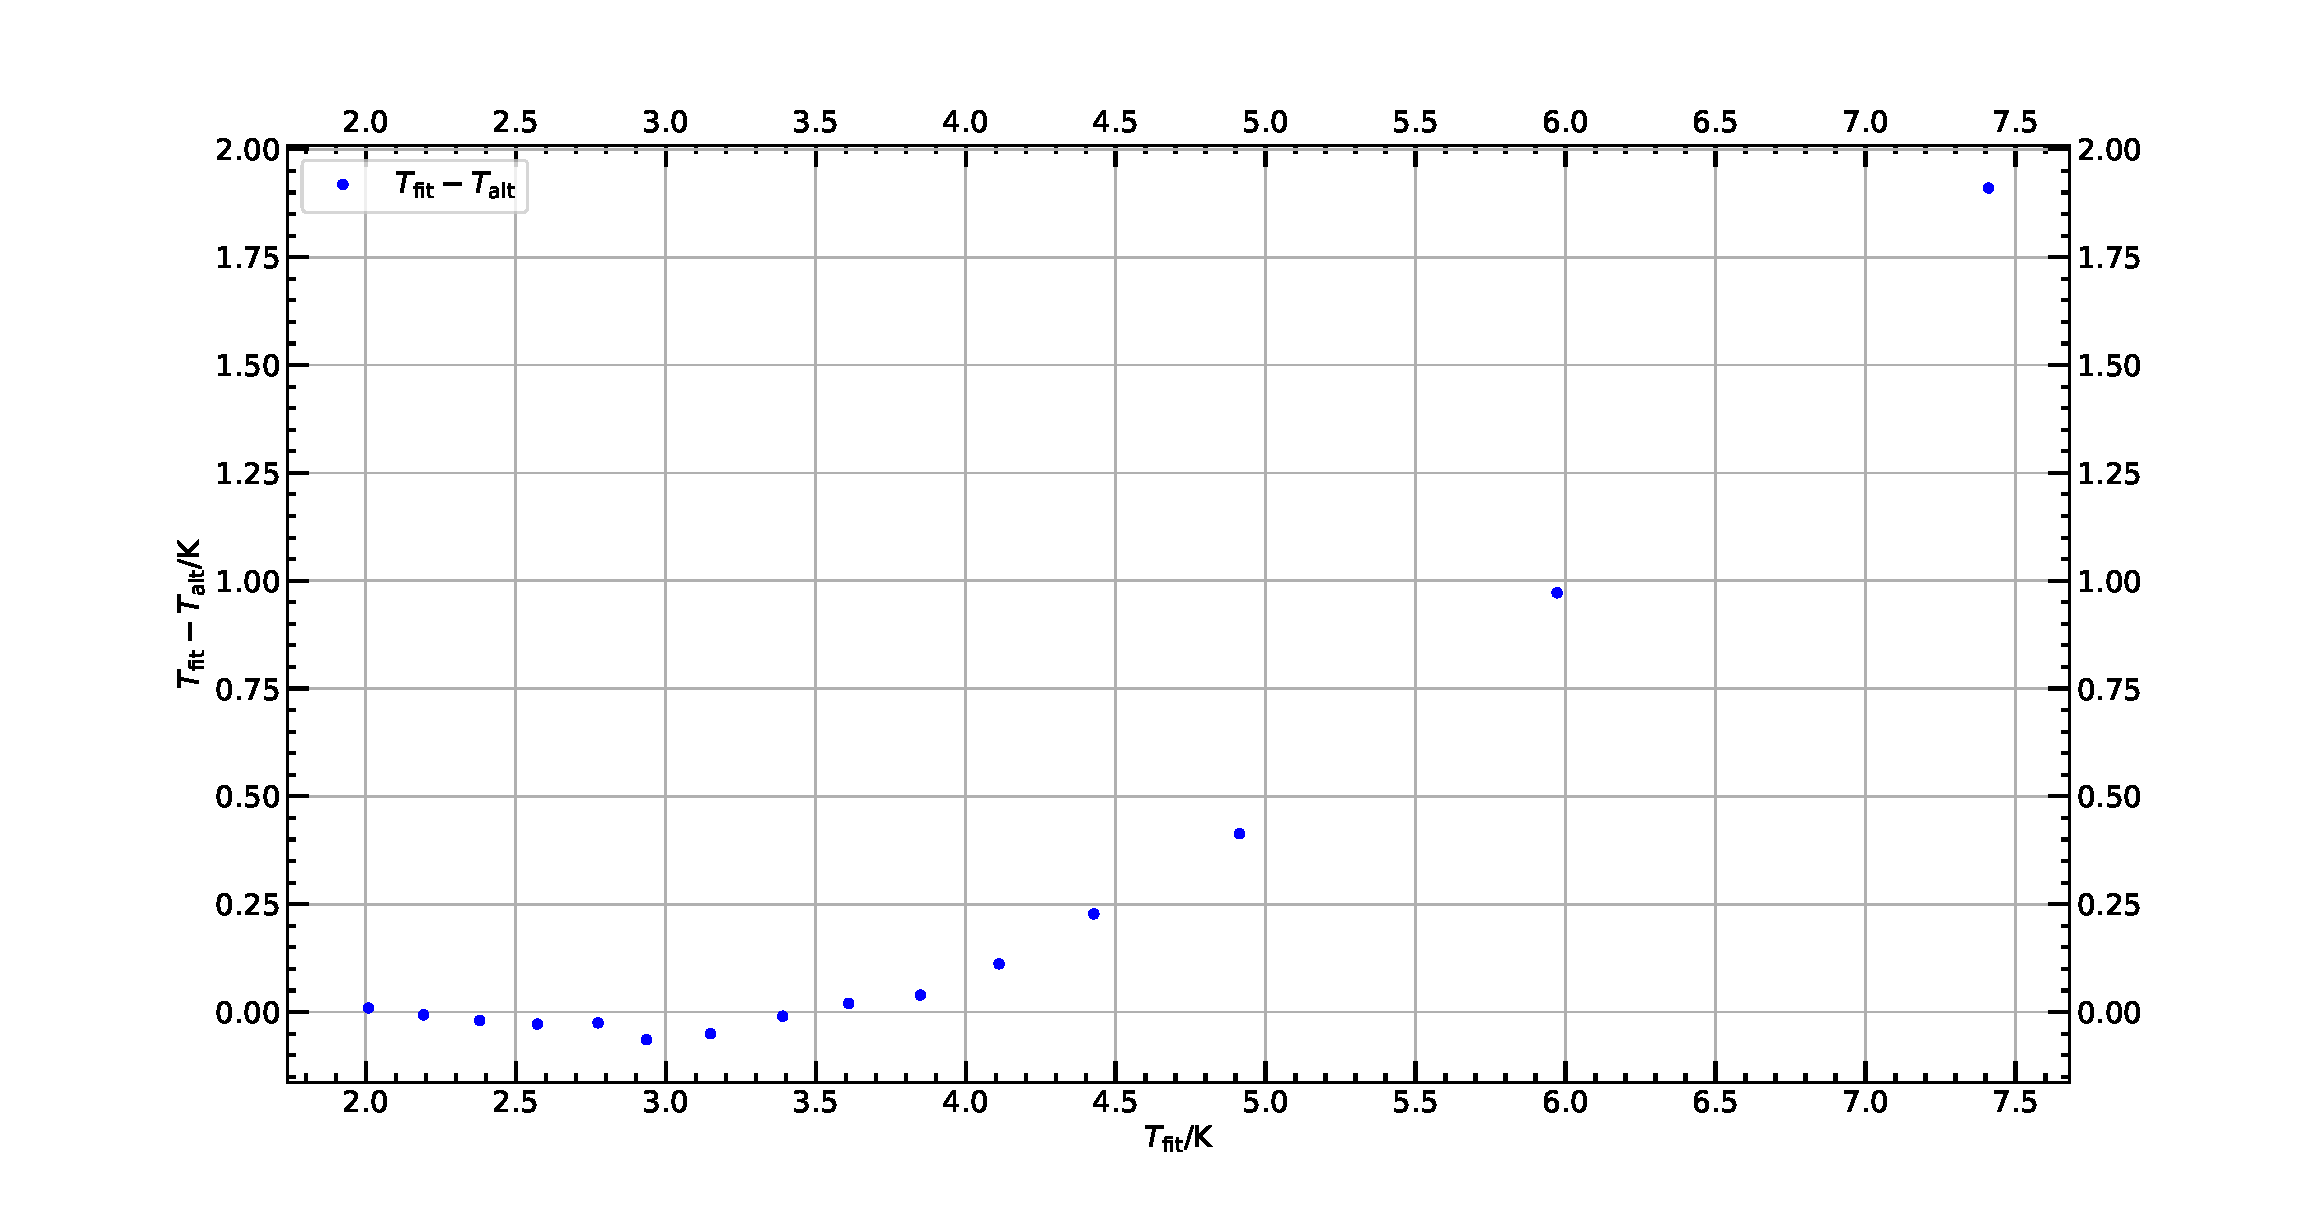
\includegraphics[width=\textwidth]{Alte_Eiche.pdf}
\caption{Vergleich der verwendeten Fitfunktion mit der alten Eichtabelle für das Germaniumthermometer.}
\end{figure}


Die Werte zeigen im Tieftemperaturbereich unterhalb von ca. \(T\approx 4 \,\mathrm{K}\) eine gute Übereinstimmung, was sich darin ausdrückt, dass die Punkte dort mit zufälligem Charakter um null streuen. Oberhalb gibt es eine deutliche Abweichung von bis zu \(\Delta T \approx 2\,\mathrm{K}\), wobei die Fitfunktion hier stets höhere Werte angibt als die Eichtabelle. Die Abweichung im Bereich höherer Temperaturen lässt sich damit erklären, dass Heißleiter einem exponentiellem Zusammenhang zwischen Widerstand und Temperatur genügen und daher für steigende Temperaturen zunehmend ungenauere Temperaturwerte liefern. Da uns im Gegensatz zu einer richtigen Eichung die genaue Beschaffenheit des Thermometers nicht bekannt ist, konnten zusätzliche Störfaktoren in unserem Fit nicht berücksichtigt werden sodass eine Abweichung von der Eichtabelle zu erwarten war.
\subsection{Vergleich aller drei Thermometer}
Um ein Gesamtbild zu erhalten, wurden die Temperatur aus dem Dampfdruckthermometer und die aus dem Germaniumthermometer über der Temperatur des dritten Thermometers dargestellt, welches man in diesem Zusammenhang als ein Messnormal ansehen kann. Die Temperatur des dritten Thermometers wird deshalb mit \(T_{\mathrm{real}}\) bezeichnet (Abbildung 18). \\\\
\begin{figure}[h!]\centering
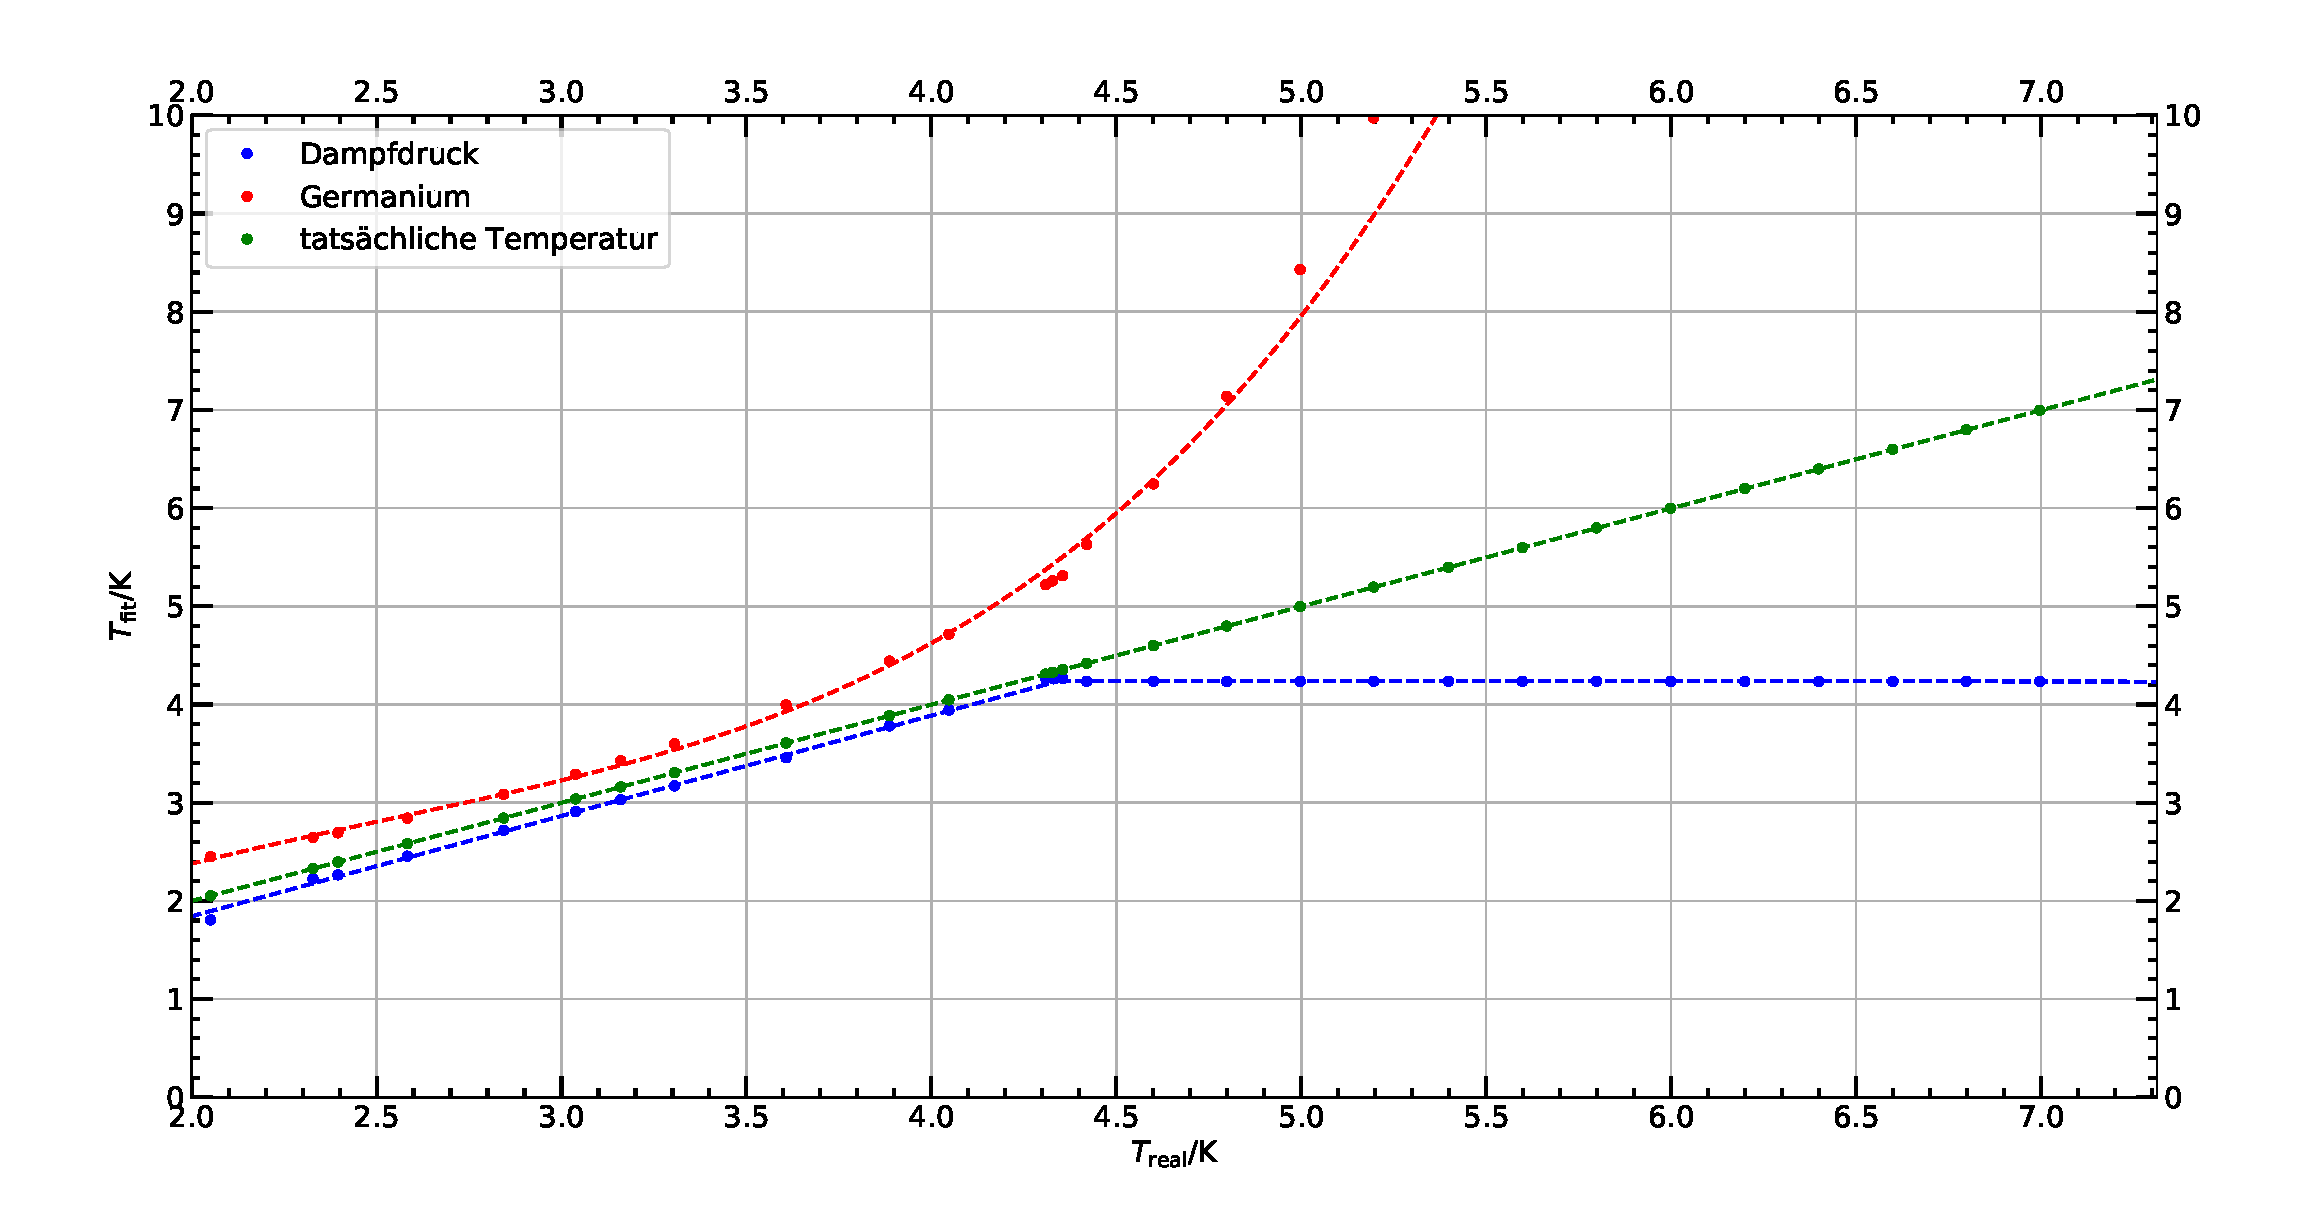
\includegraphics[width=\textwidth]{Thermometervergleich.pdf}
\caption{Vergleich der drei Thermometer. Die tatsächliche Temperatur erscheint als grüne Winkelhalbierende im Koordinatensystem.}
\end{figure}


Die Temperaturen stimmen unterhalb der Siedetemperatur von Helium recht gut mit dem Messnormal überein. Die Abweichung ist dort insbesondere systematischer Natur, weil die Kurven annähernd parallel und nur verschoben verlaufen. Oberhalb von etwa \(T\approx 4\,\mathrm{K}\) gibt es aber deutliche Abweichungen: Das Dampfdruckthermometer zeigt wie bereits erwähnt eine konstante Temperatur an, weil das Helium anfängt zu sieden. Die Kurve vom Germaniumthermometer wächst zu stark an und weicht auch im Kurvenverlauf von der Geraden ab. Dies kann, wie bereits besprochen, damit erklärt werden, dass sich Heißleiter nur für den Tieftemperaturbereich zur Widerstandsmessung eignen. 
\subsection{Werte der Gasuhr}
Wie in der Versuchsanleitung gefordert, wurde der Stand der Gasuhr bei Beginn und bei Beenden des Versuchs abgelesen. Der Startwert waren: $88.092 \,\text{m}^3$ und der Endwert: $94.263 \,\text{m}^3$. Das während des Versuchs verbrauchte Volumen an gasförmigem Helium war also: 
\begin{align*}
V(\text{GHe}) = 6.171 \, \text{m}^3.
\end{align*}
Dies kann mittels folgender Umrechnung in ein Volumen für flüssiges Helium umgerechnet werden:
\begin{align*}
700 \, \text{l} \, \text{GHe} \approx 1 \, \text{l} \, \text{LHe}.
\end{align*}
Die Umrechnung ergibt:
\begin{align*}
V(\text{LHe}) &= 6.171 \cdot 10^3 \, \text{l} \, \text{GHe} \cdot \frac{1 \, \text{l} \, \text{LHe}}{700 \, \text{l} \, \text{GHe}}. \\
\Rightarrow V(\text{LHe}) &\approx 8.82 \, \text{l}.
\end{align*}
Es wurden also während des Versuchs $8.82 \, \text{l}$ flüssiges Helium verbraucht. Dieses kann über die Heliumrückgewinnungsanlage für spätere Versuche wieder aufbereitet werden. Dies ist ökonomisch wichtig, weil flüssiges Helium sehr teuer ist.

\newpage
    % Bibliographie/Literaturverzeichnis
    \begin{thebibliography}{9}
    \bibitem{1}
    \emph{Hochtemperatursupraleiter}, \\
    \url{https://de.wikipedia.org/wiki/Hochtemperatursupraleiter#cite_note-1},
    18.\,Januar~2020.
    \bibitem{2}
    \emph{BCS-Theorie}, \\
    \url{https://de.wikipedia.org/wiki/BCS-Theorie},
    18.\,Januar~2020.
    \bibitem{3}
    Versuchsanleitung Supraleitung 2 (SU2). TU Dresden.
    \bibitem{4}
    \emph{Widerstandsthermometer}, \\
    \url{https://me-lrt.de/widerstandsthermometer},
    18.\,Januar~2020.
    \bibitem{5}
    \emph{Festkörperphysik},
    Kittel, Charles: Einführung in die Festkörperphysik. 8. Auflage. R. Oldenbourg Verlag GmbH. München. 1989.
    \bibitem{6}
    \emph{Festkörperphysik},
    Gross, Rudolf: Festkörperphysik. R. Oldenbourg Verlag GmbH. München. 2012.

    \end{thebibliography}

% Ende Dokument
\end{document}
